% SIAM Article Template
\documentclass[r]{siamart171218}
% Packages and macros go here
\usepackage[english]{babel}
\usepackage{amsmath}
\usepackage{amssymb}
\usepackage{amsfonts}
\usepackage{array}
\usepackage{graphicx}
\usepackage{epsfig}
\usepackage{float}
\usepackage{fullpage}
\usepackage{color}
\usepackage{enumitem}  
\usepackage{epstopdf}
\usepackage{stmaryrd}
\usepackage{tikz, subfigure}

\usepackage{booktabs}  % for tables
\usepackage{capt-of}
\usepackage{multirow}

\newcommand{\miro}[1]{{\color{cyan}#1}}

% Title. If the supplement option is on, then "Supplementary Material"
% is automatically inserted before the title.
%\title{On the weak coupling of 3D and 1D second order elliptic problems}
\title{Coupling PDEs on 3D-1D domains with Lagrange multipliers}

% Authors: full names plus addresses.
\author{Miroslav Kuchta, Federica Laurino, Kent-Andre Mardal, Paolo Zunino,\thanks{Authors are listed in alphabetical order}}

\begin{document}

\maketitle

% REQUIRED
\begin{abstract}
These are personal notes written to keep track of the developments on this topic, to be kept confidential.
\end{abstract}

% REQUIRED
\begin{keywords}
elliptic problems, high dimensionality gap, essential coupling conditions, Lagrange multipliers
\end{keywords}

% REQUIRED
\begin{AMS}
n.a.
\end{AMS}

% >>>>>>>>>>>>>>>>>>>>>>>>>>>>>>>>>>>>>>>>>>>>>>>>>>>>>>>>>>>>>>>>>>>>>>>>>>>>>>>>>>>>>>>>>>>>>>>>>>>>
 
% definitions here

\def\ud{u_{\odot}}
\def\vd{v_{\odot}}
\def\ld{\lambda_{\odot}}
\def\udh{u_{\odot h}}
\def\vdh{v_{\odot h}}
\def\ldh{\lambda_{\odot h}}
\def\md{\mu_{\odot}}
\def\lld{l_{\odot}}
\def\uf{u_{\ominus}}
\def\up{u_{\oplus}}
\def\eps{\epsilon}
\def\nn{\boldsymbol n}
\def\rr{\boldsymbol r}
\def\RR{\boldsymbol R}
\def\kk{\boldsymbol k}
\def\ss{\boldsymbol s}
\def\uu{\boldsymbol u}
\def\vv{\boldsymbol v}
\def\xx{\boldsymbol x}
\def\bu{\overline{u}}
\def\bv{\overline{v}}
\def\tu{\widetilde{u}}
\def\tv{\widetilde{v}}
\def\TT{\boldsymbol T}
\def\NN{\boldsymbol N}
\def\BB{\boldsymbol B}
\def\ttu{\widetilde{\widetilde{u}}}
\def\ttv{\widetilde{\widetilde{v}}}
\def\cv{\check{v}}
\def\mesh{{\cal T}^h}
\def\ball{{\cal B}}
\def\R{\mathbb{R}}
\def\D{\mathcal{D}}
\def\DD{\partial\mathcal{D}}
\def\trace{{\mathcal{T}_\Gamma}}
\def\mtrace{{\overline{\mathcal{T}}_\Lambda}}
\def\ext{\mathcal{E}_\Gamma}
\def\ide{\mathcal{I}}
\def\ii{\hat{\imath}}
\newcommand{\avrd}[1]{\overline{\overline{#1}}}
\newcommand{\avrc}[1]{\overline{#1}}
\newcommand{\refe}[1]{{#1}_{\mathrm{ref}}}
\newcommand{\norm}[1]{\lVert{#1}\rVert}

\newcommand{\vertiii}[1]{{\left\vert\kern-0.25ex\left\vert\kern-0.25ex\left\vert #1 
    \right\vert\kern-0.25ex\right\vert\kern-0.25ex\right\vert}}

\newtheorem{thm}{Theorem}[section]
\newtheorem{prop}{Property}[section]
\theoremstyle{remark}
\newtheorem{remark}{Remark}[section]
 
% >>>>>>>>>>>>>>>>>>>>>>>>>>>>>>>>>>>>>>>>>>>>>>>>>>>>>>>>>>>>>>>>>>>>>>>>>>>>>>>>>>>>>>>>>>>>>>>>>>>>
\section{Introduction}\label{sec:intro}

We address the geometrical configuration of the problem for a 3D coupled problem formulation based on from Dirichlet-Neumann interface conditions. Then, we apply a model reduction technique that transforms the problem into 3D-1D coupled PDEs. We develop and analyze a robust definition of the coupling operators form a 3D domain, $\Omega$, to 1D manifold, $\Lambda$, and vice versa. This is a non trivial objective because the standard trace operator form a domain $\Omega$ to a subset $\Lambda$ is not well posed if $\Lambda$ is a manifold of co-dimension two of $\Omega$.

% >>>>>>>>>>>>>>>>>>>>>>>>>>>>>>>>>>>>>>>>>>>>>>>>>>>>>>>>>>>>>>>>>>>>>>>>>>>>>>>>>>>>>>>>>>>>>>>>>>>>
\section{Problem setting}\label{sec:setting}

Let $\Omega \subset \mathbb{R}^3$ be a bounded, convex open set. Let $\Omega_\ominus$ be a generalized cylinder embedded into $\Omega$ and let $\Omega_\oplus = \Omega \setminus \overline{\Omega}_\ominus$ be the complementary set of the cylinder. We also introduce the set $\Lambda$, a 1D manifold that represents the centerline of $\Omega_\ominus$. We define the arc-length coordinate along $\Lambda$, denoted by $s \in (0,S)$. We denote with $\mathcal{D}(s)$ and $\partial\mathcal{D}(s)$ a cross section of $\Omega_\ominus$ and its boundary, respectively, and we assume that $\min |\D (s)| >0$, where $|\D (s)|$ is the measure of $\D (s)$. 
%In what follows, we assume for simplicity of notation that $\Sigma$ has a constant cross section, but this is not a restriction of the approach. 
We also assume that $\Omega_\ominus$ crosses $\Omega$ from side to side and we call $\Gamma$ the lateral (cylindrical) surface of $\Omega_\ominus$, while the upper and lower side faces of $\Omega_\ominus$ belong to $\partial\Omega$. We refer to Figure \ref{fig1} for an illustration of the notation. 

\begin{figure}
\begin{center}
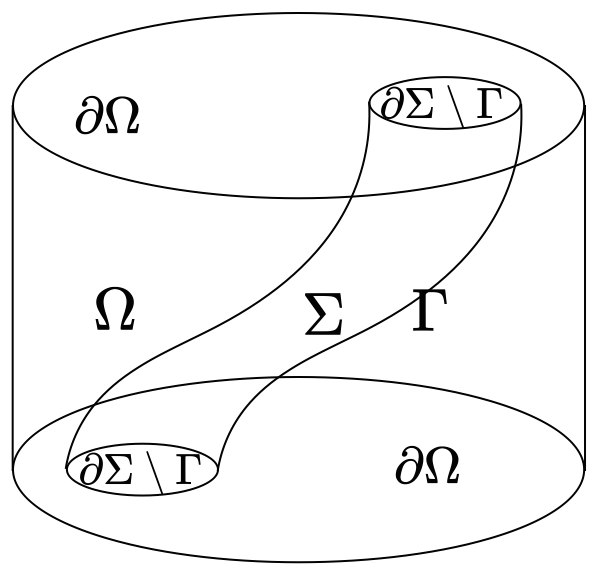
\includegraphics[width=0.5\textwidth]{3D-1D-simple.png}
\end{center}
\caption{Geometrical setting of the problem}
\label{fig1}
\end{figure}

We consider the problem arising from \emph{Dirichlet-Neumann} conditions. 
It consists to find $\up,\uf$ s.t.:
\begin{subequations}\label{eq:dirneu}
\begin{align}
\label{eq:dirneu1}
- \Delta \up  + \up &= f  && \text{ in } \Omega_{\oplus},\\
\label{eq:dirneu2}
- \Delta \uf  + \uf &= g  && \text{ in } \Omega_\ominus,\\
\label{eq:dirneu3}
-\nabla \uf \cdot \nn_{\ominus} &= -\nabla \up \cdot \nn_{\ominus}  && \text{ on } \Gamma,\\
\label{eq:dirneu4}
\uf &= \up && \text{ on }  \Gamma,\\
\label{eq:dirneu5}
\up &= 0 && \text{ on } \partial \Omega\,.
\end{align}
\end{subequations}

The objective of this work is to derive and analyze a simplified version of problem \eqref{eq:dirneu}, where the domain $\Omega_\ominus$ shrinks to its centerline $\Lambda$ and the corresponding partial differential equation is averaged on the cylinder cross section, namely $\mathcal{D}$. This new problem setting will be called the \emph{reduced} problem. Form the mathematical standpoint it is more challenging than \eqref{eq:dirneu}, because it involves the coupling of 3D/1D elliptic problems.\\

For the model reduction process, we decompose integrals as follows, for any sufficiently regular function $w$,
\begin{equation*}
\int_{\Omega_\ominus} w d\omega 
= \int_\Lambda \int_{\mathcal{D}} w d\sigma ds
= \int_\Lambda |\mathcal{D}|\avrd{w} ds\,,
\quad
\int_{\Gamma} w d\sigma 
= \int_\Lambda \int_{\partial\mathcal{D}} w d\gamma ds
= \int_\Lambda  |\partial \mathcal{D}| \avrc{w} ds\,,
\end{equation*}
where $\avrd{w}, \ \avrc{w}$ denote the following mean values respectively,
\begin{equation*}
\avrd{w} = |\mathcal{D}|^{-1} \int_{\mathcal{D}} w d\sigma\,,
\quad
\avrc{w} = |\partial\mathcal{D}|^{-1} \int_{\partial\mathcal{D}} w d\gamma\,.
\end{equation*}

We apply the model reduction approach at the level of the variational formulation.
We start from the variational formulation of problem \eqref{eq:dirneu}, 
that is to find $\up \in H^1_{\partial\Omega}(\Omega_\oplus), \ \uf \in H^1_{\partial\Omega_\ominus\setminus\Gamma}(\Omega_\ominus), \ \lambda \in H^{-\frac12}(\partial\Omega_\ominus)$ s.t.
\begin{subequations}\label{eq:weak_dirneu}
\begin{align}
&(u_\oplus,v_\oplus)_{H^1(\Omega_\oplus)} + (u_\ominus,v_\ominus)_{H^1(\Omega_\ominus)} 
+ \langle  v_\oplus - v_\ominus, \lambda \rangle_{H^{-\frac12}(\Gamma)} 
\\
\nonumber
&\qquad\qquad = (f,v_\oplus)_{L^2(\Omega_\oplus)} + (g,v_\ominus)_{L^2(\Omega_\ominus)}
\quad \forall v_\oplus \in H^1_{\partial\Omega}(\Omega_\oplus), \ v_\ominus \in H^1_{\partial\Omega_\ominus\setminus\Gamma}(\Omega_\ominus)
\\
& \langle u_\oplus - u_\ominus, \mu \rangle_{H^{-\frac12}(\Gamma)} = 0
\quad \forall  \mu \in H^{-\frac12}(\Gamma)\,,
\end{align}
\end{subequations}
where $\langle v, \mu \rangle_{H^{-\frac12}(\Gamma)}$ denotes the duality pairing between 
$ \mu \in H^{-\frac12}(\Gamma)$ and $v \in H^{\frac12}(\Gamma)$.
In this case, the additional variable $\lambda$ is equivalent to $\lambda  =  \nabla \uf \cdot \nn_\ominus$.

Using a model reduction approach based on averaging, we end up with two different formulations of a reduced problem
for the unknown $u$ defined on the entire 3D domain $\Omega$, coupled with the unknown $\ud$, defined on the 1D manifold $\Lambda$
and a Lagrange multiplier defined either on $\Gamma$ (problem 1) or on $\Lambda$ (problem 2). 
The scope of this work is to compare them, with the aim to determine which is the most suitable to set up a computational model for 3D-1D PDEs coupled with Dirichlet-Neumann constraint.


% >>>>>>>>>>>>>>>>>>>>>>>>>>>>>>>>>>>>>>>>>>>>>>>>>>>>>>>>>>>>>>>>>>>>>>>>>>>>>>>>>>>>>>>>>>>>>>>>>>>>
\subsection{Topological model reduction}
\subsubsection*{Model reduction of the problem on $\Omega_{\ominus}$}

We apply the averaging technique to equation \eqref{eq:dirneu2}. In particular, we consider an arbitrary portion $\mathcal{P}$ of the cylinder $\Omega_\ominus$, with lateral surface $\Gamma _{\mathcal{P}}$ and bounded by two perpendicular sections to $\Lambda$, namely $\mathcal{D}(s_1), \ \mathcal{D}(s_2)$ with $s_1<s_2$. We have,
\begin{multline*}
\int_{\mathcal{P}} -\Delta \uf + \uf d\omega =
-\int_{\partial \mathcal{P}} \nabla \uf \cdot \nn_{\ominus} \, d\sigma  + \int_{\mathcal{P}}\uf d\omega=
\\
 \int_{\mathcal{D}(s_1)} \partial_s \uf d\sigma -  \int_{\mathcal{D}(s_2)} \partial_s \uf d\sigma -  \int_{\Gamma_{\mathcal{P}}} \nabla \uf \cdot \nn_{\ominus} d\sigma +\int_{\mathcal{P}}\uf d\omega
\end{multline*}
By the fundamental theorem of integral calculus combined with the Reynolds transport Theorem, 
being $\nu$ the normal deformation of the boundary along $(0,S)$, we have,
\begin{equation*}
\begin{split}
\int_{\mathcal{D}(s_1)} \partial_s \uf d\sigma -  \int_{\mathcal{D}(s_2)} \partial_s \uf d\sigma 
&= -\int_{s_1}^{s_2} d_s \int_{\mathcal{D}(s)}  \partial_s \uf d\sigma ds
\\
&= -\int_{s_1}^{s_2} d_{ss}^2 \int_{\D(s)} u_{\ominus} \, d\sigma \, ds +  \int_{s_1}^{s_2} d_s \left( \int_{\DD(s)} \nu u_{\ominus} \, d\gamma \right) ds\,,
\end{split}
\end{equation*}
and assuming that $\D(s)$  can not change shape, we have
\begin{equation*}
\begin{split}
-\int_{s_1}^{s_2} d_{ss}^2 \int_{\D(s)} u_{\ominus} \, d\sigma \, ds + \int_{s_1}^{s_2} d_s \left( \int_{\DD(s)} \nu u_{\ominus} \, d\gamma \right)\, ds
&=-\int_{s_1}^{s_2} \left[d_{ss}^2 (|\D(s)|\avrd{u}_{\ominus}) -  d_s(  \nu |\DD(s)| \avrc{u}_{\ominus} ) \right] \, ds
\\
&=-\int_{s_1}^{s_2} \left[d_{ss}^2 (|\D(s)|\avrd{u}_{\ominus}) -  d_s\left(d_s(|\D(s)|) \avrc{u}_{\ominus} \right) \right] \, ds.
\end{split}
\end{equation*}
Moreover, we have
\begin{equation*}
\int_{\Gamma_{\mathcal{P}}} \nabla \uf \cdot \nn_{\ominus} d\sigma =  \int_{\Gamma_{\mathcal{P}}} \lambda \, d\sigma
=  \int_{s_1}^{s_2} \int_{\partial\mathcal{D}(s)} \lambda d\gamma \, ds 
= \int_{s_1}^{s_2} |\DD| \avrc{\lambda} \,ds\,.
\end{equation*}
From the combination of all the above terms with the right hand side, we obtain that the solution $\uf$ of \eqref{eq:dirneu2} satisfies,
\begin{equation*}
\int_{s_1}^{s_2} \left[ 
-d_{ss}^2 (|\D(s)|\avrd{u}_{\ominus}) +  d_s\left(d_s(|\D(s)|) \avrc{u}_{\ominus}\right) + |\D(s)|\avrd{u}_{\ominus} 
- |\partial\mathcal{D}(s)| \avrc{\lambda} 
\right] \, ds = \int_{s_1}^{s_2} |\mathcal{D}(s)| \avrd{g}\, ds \,.
\end{equation*}
Since the choice of the points $s_1,s_2$ is arbitrary, we conclude that the following equation holds true,
\begin{equation}\label{eq:averaged_f}
-d_{ss}^2 (|\D(s)|\avrd{u}_{\ominus}) +  d_s\left(d_s(|\D(s)|) \avrc{u}_{\ominus}\right) + |\D(s)|\avrd{u}_{\ominus} 
- |\partial\mathcal{D}(s)| \avrc{\lambda}
= |\mathcal{D}(s)| \avrd{g} \quad \text{on} \ \Lambda\,,
\end{equation}
which is complemented by the following conditions at the boundary of $\Lambda$,
\begin{equation}\label{eq:averaged_f_boundary}
|\D(s)| d_s \avrd{u}_{\ominus} = 0, \quad d_s |\D(s)| = 0, \quad \text{on} \quad s=0,S.
\end{equation}
Then, we consider variational formulation of the averaged equation \eqref{eq:averaged_f}.
After multiplication by a test function $\vd \in H^1(\Lambda)$, integration on $\Lambda$ and suitable application of integration by parts, we obtain,
\begin{multline*}
\int_\Lambda d_s (|\D(s)| \avrd{u}_{\ominus} ) d_s \vd \, ds - d_s (|\D(s)| \avrd{u}_{\ominus} ) \vd |_{s=0}^{s=S}
- \int_\Lambda (d_s |\D(s)|)\avrc{u}_{\ominus} d_s \vd \, ds + (d_s |\D(s)|) \avrc{u}_{\ominus} \vd |_{s=0}^{s=S}
\\
+\int_\Lambda |\D(s)| \avrd{u}_\ominus \vd - \int_\Lambda |\DD(s)| \avrc{\lambda} \vd \, ds
= \int_\Lambda |\D(s)| \avrd{g} V\, ds\,.
\end{multline*}
Using boundary conditions, 
the identity $d_s (|\D(s)| \avrd{u}_{\ominus} ) = |\D(s)| d_s \avrd{u}_{\ominus} + d_s (|\D(s)|) \avrd{u}_{\ominus}$
and reminding that $d_s |\D(s)|)/|\DD(s)| = \nu$,
we obtain,
\begin{equation}\label{eq:averaged_f_weak}
(d_s \avrd{u}_{\ominus}, d_s \vd )_{\Lambda,|\D|} 
+ ( \nu (\avrd{u}_{\ominus} - \avrc{u}_{\ominus}), d_s \vd)_{\Lambda,|\DD|} +(\avrd{u}_\ominus, \vd)_{\Lambda, |\D|}
- (\avrc{\lambda},\vd)_{\Lambda,|\DD|}
= (\avrd{g},V)_{\Lambda,|\D|}\,.
\end{equation}
where we have introduced the following weighted inner product notation,
\begin{equation*}
(\ud,\vd)_{\Lambda,w} = \int_0^S w(s) \ud(s) \vd(s) ds\,.
\end{equation*}
Let us now formulate the modelling assumption that allows us to reduce equation \eqref{eq:averaged_f_weak} to a solvable one-dimensional (1D) model.
More precisely, we assume that:
\begin{description}
\item[A1] the function $\uf$ has a \emph{uniform profile} on each cross section $\mathcal{D}(s)$, namely $\uf(r,s,t) = \ud(s)$.
\end{description}
Therefore, observing that $\ud=\avrc{u}_{\ominus}=\avrd{u}_{\ominus}$, problem \eqref{eq:averaged_f_weak} consists to find $\ud \in H^1(\Lambda)$ such that
\begin{equation}\label{eq:1Ddirneu_weak}
 (d_s \ud, d_s \vd)_{\Lambda,|\mathcal{D}|} 
+(\ud, \vd)_{\Lambda, |\D|}
-(\avrc{\lambda},\vd)_{\Lambda, |\DD|}
=  (\avrd{g},\vd)_{\Lambda, |\mathcal{D}|}
\quad \forall \vd \in H^1(\Lambda)\,.
\end{equation}

% >>>>>>>>>>>>>>>>>>>>>>>>>>>>>>>>>>>>>>>>>>>>>>>>>>>>>>>>>>>>>>>>>>>>>>>>>>>>>>>>>>>>>>>>>>>>>>>>>>>>
\subsubsection*{Topological model reduction of the problem on $\Omega_{\oplus}$}
We focus here on the subproblem of \eqref{eq:dirneu1} related to $\Omega_{\oplus}$.
We multiply both sides of \eqref{eq:dirneu1} by a test function $v\in H^1_0(\Omega)$ and integrate on $\Omega_\oplus$. Integrating by parts and using boundary and interface conditions, we obtain
\begin{equation*}
\begin{split}
\int_{\Omega _{\oplus}}fv\,d\omega&=
\int _{\Omega _{\oplus}}\nabla \up \cdot\nabla v\,d\omega -\int _{\partial \Omega _{\oplus}}\nabla \up \cdot \nn_{\oplus} v\,d\sigma + \int_{\Omega_{\oplus}} \up v
\\
&=\int _{\Omega _{\oplus}}\nabla \up \cdot\nabla v\,d\Omega -\int_{\Gamma} \nabla \up \cdot \nn_{\oplus} v + \int_{\Omega_{\oplus}} \up v
\\
&=\int _{\Omega _{\oplus}}\nabla \up \cdot\nabla v\,d\Omega +\int_{\Gamma} \lambda v + \int_{\Omega_{\oplus}} \up v.
\end{split}
\end{equation*} 
Then, we make the following modelling assumptions:
\begin{description}
\item[A2] we identify the domain $\Omega_{\oplus}$ with the entire $\Omega$, 
and we correspondingly omit the subscript $\oplus$ to the functions defined on $\Omega_{\oplus}$,
namely
\begin{equation*}
\int_{\Omega_{\oplus}} u_\oplus\, d\omega \simeq \int_{\Omega} u\, d\omega\,.
\end{equation*}
\end{description}
Therefore, we obtain 
\begin{equation*}
(\nabla u ,\nabla v)_{\Omega} +(u,v)_{\Omega}+(\lambda, v)_{\Gamma}  =(f,v)_{\Omega}
\end{equation*}
and combining with \eqref{eq:1Ddirneu_weak} we obtain the first formulation of the reduced problem.

\subsubsection*{Problem 1 (3D-2D-1D)}
Let $\langle \cdot , \cdot \rangle_\Gamma$ denote the duality pairing between 
$H^\frac12_{00}(\Gamma)$ and $H^{-\frac12}(\Gamma)$. The problem consists to find $u \in H^1_0(\Omega), \ \lambda \in H^{-\frac12}(\Gamma ),\ \ud \in H^1_0(\Lambda)$, such that
\begin{subequations}\label{eq:problem1}
\begin{align}
&(u,v)_{H^1(\Omega)} + (\ud,\vd)_{H^1(\Lambda),|\D|} 
+ \langle \trace v  - \ext \vd, \lambda \rangle_\Gamma
\\
\nonumber
&\qquad\qquad= (f,v)_{L^2(\Omega)} +  (\avrd{g},\vd)_{L^2(\Lambda),|\D|}
\quad \forall v \in H^1_0(\Omega), \ \vd \in H^1(\Lambda)
\\
&   \langle \trace u - \ext \ud , \mu \rangle_\Gamma = 0
\quad \forall \mu \in H^{-\frac12}(\Gamma)\,.
\end{align}
\end{subequations}
Here, $\trace:H^1_0(\Omega) \rightarrow H^{\frac 12}_{00}(\Gamma)$ denotes the trace operator from $\Omega$ to $\Gamma$ and $\ext: H^1_0(\Lambda) \rightarrow H^1_{0}(\Gamma)$ denotes the uniform extension from $\Lambda$ to $\Gamma$ and we exploited the fact that 
\begin{equation*}
\left( \avrc{\lambda}, \vd \right)_{\Lambda, |\DD|} 
= \int _{\Lambda} |\DD| \left( \frac{1}{|\DD|} \int_{\DD} \lambda \, d\gamma \right) \vd \, ds 
= (\lambda, \ext \vd)_{\Gamma}.
\end{equation*} 

% >>>>>>>>>>>>>>>>>>>>>>>>>>>>>>>>>>>>>>>>>>>>>>>>>>>>>>>>>>>>>>>>>>>>>>>>>>>>>>>>>>>>>>>>>>>>>>>>>>>>
Now, we apply a topological model reduction of the interface conditions, namely we go from a 3D-2D-1D formulation
involving sub-problems on $\Omega$ and $\Lambda$ and coupling operators defined on $\Gamma$
to a 3D-1D-1D formulation where the coupling terms are set on $\Lambda$. 
To this purpose, let us write the Lagrange multiplier and the test functions on every cross section $\partial\mathcal{D}(s)$ as their average plus some fluctuation,
\begin{equation*}
\lambda=\avrc{\lambda}+\tilde{\lambda}, \qquad v=\avrc{v}+\tilde{v},
\quad \text{on} \ \partial\mathcal{D}(s)\,,
\end{equation*}
where $\avrc{\tilde{\lambda}}=\avrc{\tilde{v}}=0$. 
Therefore, the coupling term on $\Gamma$ can be decomposed as,
\begin{equation*}
\int_{\Gamma}\lambda v\, d\sigma
=\int _{\Lambda}  \int_{\partial\mathcal{D}(s)} (\avrc{\lambda}+\tilde{\lambda})(\avrc{v}+\tilde{v})d\gamma ds
= \int_{\Lambda}|\partial\mathcal{D}(s)| \avrc{\lambda}\avrc{v}\,ds+\int_{\Lambda}  \int_{\partial\mathcal{D}(s)} \tilde{\lambda}\tilde{v}d\gamma ds\,.
\end{equation*}

Then, we make the following modelling assumptions:
\begin{description}
\item[A3] we assume that the product of fluctuations is small, namely
\begin{equation*}
\int_{\partial\mathcal{D}(s)} \tilde{\lambda}\tilde{v} d\gamma \simeq 0\,
\end{equation*}
\end{description}
and the term $\left(\trace v, \lambda \right)_{\Gamma}$ becomes $\left( \mtrace v, \avrc{\lambda} \right)_{\Lambda, |\DD|}$, where $\mtrace$ denotes the composition of operators $\trace \circ \avrc{(\cdot)}$.  Combined with \eqref{eq:1Ddirneu_weak}, this leads to the second formulation of the reduced problem.

\subsubsection*{Problem 2 (3D-1D-1D)}
Let $\langle \cdot , \cdot \rangle_\Lambda$ denote the duality pairing between 
$H^\frac12_{00}(\Lambda)$ and $H^{-\frac12}(\Lambda)$.
The problem requires to find $u \in H^1_0(\Omega),\ \ud \in H^1_0(\Lambda), \ \ld \in H^{-\frac12}(\Lambda)$, such that
\begin{subequations}\label{eq:problem2}
\begin{align}
&(u,v)_{H^1(\Omega)} + (\ud,\vd)_{H^1(\Lambda),|\D|} 
+  \langle \mtrace v - \vd, \ld \rangle_{H^{-\frac12}(\Lambda), |\DD|} 
\\
\nonumber
&\qquad\qquad= (f,v)_{L^2(\Omega)} +  (\avrd{g},V)_{L^2(\Lambda),|\D|}
\quad \forall v \in H^1_0(\Omega), \ \vd \in H^1_0(\Lambda)\,,
\\
&   \langle \mtrace u -   \ud, \md \rangle_{H^{-\frac12}(\Lambda),|\DD|} = 0
\quad \forall \md \in H^{-\frac12}(\Lambda)\,,
\end{align}
\end{subequations}
where $\mtrace$ denotes the composition of operators $\trace \circ \avrc{(\cdot)}$.
We notice that all the integrals of the reduced problem are well defined because 
$\mtrace: H^1_0(\Omega) \rightarrow H^\frac12_{00}(\Lambda)$ as shown in the following.\\

%\begin{lemma}\label{lemma:H12norm}
%{\color{red}TO DO: generalize to not uniform $\DD$} 
%When $\Gamma$ is a cylinder, if $u\in H_{00}^{\frac 12}(\Gamma)$, then $\avrc{u}\in H_{00}^{\frac 12}(\Lambda)$. Moreover, if $u\in H^{\frac 12}_{00}(\Gamma)$ is constant on each cross section, namely $u(s,\theta)=u(s)$, then 
%\begin{equation*}
%\|u\|_{H^{\frac 12}_{00}(\Gamma)}=2\pi R \|u\|_{H^{\frac 12}_{00}(\Lambda)}.
%\end{equation*}
%\end{lemma}
%\begin{proof}
%Let us denote as $\phi _{ij}$ and $\rho _{ij}$, for $i=1,2,\dots$, $j=0,1,\dots$, the eigenfunctions and the eigenvalues of the laplacian on $\Gamma$, and with $\phi _i$ and $\rho _i$ the eigenfunctions and the eigenvalues of the laplacian on $\Lambda$. In particular,
%\begin{align*}
%\phi _{ij}(s,\theta)=sin (i\pi s)\left( cos(j\theta)+ sin(j\theta) \right),\\
%\rho_{ij}=i\pi ^2+\frac{j^2}{R^2},\\
%\phi _{i}(s)=sin (i\pi s),\\
%\rho _i = i\pi ^2.
%\end{align*}
%It is easy to verify that 
%\begin{eqnarray}
%\label{null_int_eigenf}
%\int_0^{2\pi} \phi _{ij}(s,\theta)=0 \quad \forall j>0, \forall i \\
%\label{nonull_int_eigenf}
%\int_0^{2\pi} \phi _{ij}(s,\theta)= 2\pi R \, \sin(i \pi s) \quad \mbox{if } j=0, \forall i  .\\
%\end{eqnarray}
%Moreover we recall that $\phi_{i,j}(s,\theta)$ and $\phi _i(s)$ are orthogonal basis of $L^2(\Gamma)$ and $L^2(\Lambda)$ respectively. Therefore,
%\begin{multline*}
%\avrc{u}(s)=\frac{1}{2\pi R}\int_0^{2\pi} u(s,\theta)R\, d\theta
%= \frac{1}{2\pi R}\int_0^{2\pi} \sum_{i,j} a_{i,j} \phi_{i,j}(s,\theta) R\, d\theta
%\\= \frac{1}{2\pi R}\sum_{i,j} a_{i,j}\int_0^{2\pi}  \phi_{i,j}(s,\theta) R\, d\theta
%=  \sum_{i} a_{i,0} \phi_{i}(s).
%\end{multline*}
%From \cite[Lemma 4.11]{chandler2015interpolation} we have
%\begin{equation}\label{H12norm_Gamma}
%\|u\|^2_{H^{\frac 12}(\Gamma)}=\sum_{i=1}^{\infty}\sum_{j=0}^{\infty} \left( 1+ \rho_{ij}\right)^{\frac 12}|a_{ij}|^2,
%\text{ with }
%a_{ij}=\int _0^1\int _0^{2\pi} u(s,\theta )\phi_{ij}\, R d\theta ds.
%\end{equation}
%and 
%\begin{equation*}
%\|\avrc{u}\|^2_{H^{\frac 12}(\Lambda)}=\sum_{i=1}^{\infty} \left( 1+ \rho_{i}\right)^{\frac 12}|\avrc{a}_i|^2,
%\text{ with }
%\avrc{a}_i=\int _0^1 \avrc{u}(s )\phi_{i}(s) ds.
%\end{equation*}
%
%Therefore, we have
%\begin{multline*}
%\|\avrc{u}\|^2_{H^{\frac 12}(\Lambda)}=
%\sum_{i=1}^{\infty}\left( 1+ i^2\pi^2\right)^{\frac 12}\left( \int_0^1 \avrc{u}(s) sin(i\pi s)\, ds \right)^2\\
%= \sum_{i=1}^{\infty} \left( 1+ i^2\pi^2\right)^{\frac 12}\left( \sum_{j=1}^\infty a_{j,0}\int_0^1 \sin(j\pi s) \sin(i\pi s) \, ds  \right)^2\\
%= \sum_{i=1}^{\infty} \frac 14 \left( 1+ i^2\pi^2\right)^{\frac 12}a_{i,0}^2\\
%\leq \sum_{i=1}^{\infty} \sum_{j=1}^{\infty}  \left( 1+ i^2\pi^2 + \frac{j^2}{R^2}\right)^{\frac 12} |a_{i,j}|^2 =\|u\|^2_{H^{\frac 12}(\Gamma)},
%\end{multline*}
%
%where we have used the fact that
%\begin{eqnarray*}
%&\int_0^1 \sin(i\pi s) \sin(j\pi s)\, ds=0 \quad \text{if $i\neq j$}\\
%&\int_0^1 \sin(i\pi s) \sin(j\pi s)\, ds=\frac 12 \quad \text{if $i =j$}.
%\end{eqnarray*}
%Moreover, in the case in which $u$ is constant on each cross section, from \eqref{H12norm_Gamma} we have
%\begin{multline*}
%\|u\|^2_{H^{\frac 12}(\Gamma)}=\sum_{i=1}^{\infty}\sum_{j=0}^{\infty} \left( 1+ \rho_{ij}\right)^{\frac 12}|a_{ij}|^2
%=\sum_{i=1}^{\infty}\sum_{j=0}^{\infty} \left(  1+ i\pi ^2+\frac{j^2}{R^2}\right)^{\frac 12}\left( \int _0^1\int _0^{2\pi} u(s,\theta )\phi_{ij}\, R d\theta ds \right)^2\\
%=\sum_{i=1}^{\infty}\sum_{j=0}^{\infty} \left(  1+ i\pi ^2+\frac{j^2}{R^2}\right)^{\frac 12}\left( \int _0^1 u(s) \int _0^{2\pi} \phi_{ij}\, R d\theta ds \right)^2,
%\end{multline*}
%and using \eqref{null_int_eigenf} and \eqref{nonull_int_eigenf}, we obtain
%\begin{multline*}
%\|u\|^2_{H^{\frac 12}(\Gamma)}=
%\sum_{i=1}^{\infty}\left( 1+ i\pi ^2\right)^{\frac 12}\left(\int _0^1 u(s )sin (i\pi s) 2\pi R ds\right)^2\\
%=4\pi ^2 R^2 \sum_{i=1}^{\infty}\left( 1+ \rho _i\right)^{\frac 12}|a_i|^2 = 4\pi ^2 R^2  \|u\|^2_{H^{\frac 12}(\Lambda)}.
%\end{multline*}
%\hspace*{0.9\textwidth} c.v.d.
%\end{proof}
%\begin{remark}
%The results of \eqref{lemma:H12norm}  can be generalized to the case of a  different geometry of $\Gamma$, for example a parallelepiped.  
%\end{remark}

From the theory of interpolation of Sobolev spaces  illustrated in \cite{chandler2015interpolation}, we can define the fractional norms $\|\cdot \|_{H^{\frac 12}(\Gamma)}$ and $\|\cdot \|_{H^{\frac 12}(\Lambda)}$ as functions of the eigenvalues and eigenfunctions of the Laplacian on $\Gamma$ and $\Lambda$ respectively. In particular, from \cite[Lemma 4.11]{chandler2015interpolation}, if we denote as $\phi _{ij}$ and $\rho _{ij}$, for $i=1,2,\dots$, $j=0,1,\dots$, the eigenfunctions and the eigenvalues of the Laplacian on $\Gamma$ with homogeneous Dirichlet condition at the boundary, for any function $u \in H^{\frac 12}_{00}(\Gamma)$ we have
\begin{equation}\label{eq:fracnorm_gamma}
\|u\|_{H^{\frac 12}(\Gamma)}=\left(\sum_{i=1}^{\infty}\sum_{j=0}^{\infty} \left( 1+ \rho_{ij}\right)^{\frac 12}|a_{ij}|^2\right)^{\frac 12},
\text{ with }
a_{ij}=\left( u,\phi _{ij} \right)_{\Gamma}.
\end{equation}
Similarly, denoting with $\phi _i$ and $\rho _i$ the eigenfunctions and the eigenvalues of the Laplacian on $\Lambda$ with homogenous Dirichlet boundary conditions, if $u \in H^{\frac 12}(\Lambda)$ we have
\begin{equation}\label{eq:fracnorm_lambda}
\|u\|_{H^{\frac 12}_{00}(\Lambda)}=\left(\sum_{i=1}^{\infty} \left( 1+ \rho_{i}\right)^{\frac 12}|a_i|^2\right)^{\frac 12},
\text{ with }
a_i=\left(u, \phi _i \right)_{\Lambda}.
\end{equation}
In the same way, we can define the equivalent weighted norm in $H^{\frac 12}_{00}(\Lambda)$
\begin{equation}\label{eq:weightfracnorm}
\|u\|_{H^{\frac 12}_{00}(\Lambda), |\DD|}=\left(\sum_{i=1}^{\infty} \left( 1+ \rho_{i}\right)^{\frac 12}|a_i|^2\right)^{\frac 12},
\text{ with }
a_i=\left(u, \phi _i \right)_{\Lambda, |\DD|}.
\end{equation}

\begin{lemma}\label{lemma:H12norm}
Let $\Gamma$ be a tensor product domain, $\Gamma= (0,X) \times (0,Y)$. For any regular $u(x,y)$ in $\Gamma$, let $\avrc{u}(x)=\frac 1Y \int _0^Y u(x,y)\, dy$. Then, for any $u\in H_{00}^{\frac 12}(\Gamma)$, then $\avrc{u}(x)\in H_{00}^{\frac 12}((0,X))$. 
Moreover, if $u(x,y)\in H^{\frac 12}_{00}(\Gamma)$ is constant with respect to $y$, namely $u(x,y)=u(x)$, then 
\begin{equation*}
\|u\|_{H^{\frac 12}_{00}(\Gamma)}=Y \|u\|_{H^{\frac 12}_{00}(0,X)}.
\end{equation*}
\end{lemma}
\begin{proof}
In order to apply \eqref{eq:fracnorm_gamma} and \eqref{eq:fracnorm_lambda}, let us consider the eigenvalue problems for the Laplace operator on $\Gamma$ with homogeneous Dirichlet conditions at $x=0,\, X$ and periodic boundary conditions at $y=0,\, Y$. Let us also consider the Laplace eigeinproblem on $(0,X)$ with homogeneous Dirichlet conditions. Let us denote as $\phi _{ij}(x,y)$ and $\rho _{ij}$, for $i=1,2,\dots$, $j=0,1,\dots$, the eigenfunctions and the eigenvalues of the Laplacian on $\Gamma$, and with $\phi _i(x)$ and $\rho _i$ the eigenfunctions and the eigenvalues of the laplacian on $(0,X)$. In particular,
\begin{align*}
\phi _{ij}(x,y)=\sin \left(\frac{i\pi x}{X}\right)\left( cos\left(\frac{j2\pi y}{Y}\right)+ sin	\left(\frac{j2\pi y}{Y}\right) \right),\\
\rho_{ij}=\left(\frac{i\pi}{X}\right) ^2+\left(\frac{j2\pi}{Y}\right)^2,\\
\phi _{i}(x)=\sin \left(\frac{i\pi x}{X}\right),\\
\rho _i = \left(\frac{i\pi}{X}\right) ^2.
\end{align*}
It is easy to verify that 
\begin{eqnarray}
\label{null_int_eigenf}
\int_0^{Y} \phi _{ij}(x,y)=0 \quad \forall j>0, \forall i \\
\label{nonull_int_eigenf}
\int_0^{Y} \phi _{ij}(x,y)= Y \, \sin\left(\frac{i\pi x}{X}\right) \quad \mbox{if } j=0, \forall i  .
\end{eqnarray}
Moreover we recall that $\phi_{i,j}(x,y)$ and $\phi _i(x)$ form an orthogonal basis of $L^2(\Gamma)$ and $L^2(0,X)$ respectively. Therefore,
\begin{multline*}
\avrc{u}(x)=\frac{1}{Y}\int_0^{Y} u(x,y)\, dy
= \frac{1}{Y}\int_0^{Y} \sum_{i,j} a_{i,j} \phi_{i,j}(x,y) \, dy
\\= \frac{1}{Y}\sum_{i,j} a_{i,j}\int_0^{Y}  \phi_{i,j}(x,y) \, dy
=  \sum_{i} a_{i,0} \phi_{i}(x).
\end{multline*}
%From \cite[Lemma 4.11]{chandler2015interpolation} we have
%\begin{equation}\label{H12norm_Gamma}
%\|u\|^2_{H^{\frac 12}(\Gamma)}=\sum_{i=1}^{\infty}\sum_{j=0}^{\infty} \left( 1+ \rho_{ij}\right)^{\frac 12}|a_{ij}|^2,
%\text{ with }
%a_{ij}=\int _0^X\int _0^{Y} u(x,y )\phi_{ij} (x,y)dy dx.
%\end{equation}
%and 
%\begin{equation*}
%\|\avrc{u}\|^2_{H^{\frac 12}(0,X)}=\sum_{i=1}^{\infty} \left( 1+ \rho_{i}\right)^{\frac 12}|\avrc{a}_i|^2,
%\text{ with }
%\avrc{a}_i=\int _0^X \avrc{u}(x )\phi_{i}(x) dx.
%\end{equation*}

From \eqref{eq:fracnorm_lambda} we have
\begin{multline*}
\|\avrc{u}\|^2_{H^{\frac 12}(0,X)}
=\sum_{i=1}^{\infty} \left( 1+ \rho_{i}\right)^{\frac 12}a_i^2\\
=\sum_{i=1}^{\infty}\left( 1+ \left(\frac{i\pi}{X}\right)^2\right)^{\frac 12}\left( \int_0^X \avrc{u}(x) \sin\left(\frac{i\pi x}{X}\right)\, dx \right)^2\\
= \sum_{i=1}^{\infty} \left( 1+ \left(\frac{i\pi}{X}\right)^2\right)^{\frac 12}\left( \sum_{j=1}^\infty a_{j,0}\int_0^X \sin\left(\frac{j\pi x}{X}\right) \sin\left(\frac{i\pi x}{X}\right) \, dx  \right)^2\\
= \sum_{i=1}^{\infty} \frac{X^2}{4} \left( 1+ \left(\frac{i\pi}{X}\right)^2\right)^{\frac 12}a_{i,0}^2\\
\leq \frac{X^2}{4}\sum_{i=1}^{\infty} \sum_{j=1}^{\infty}  \left( 1+ \left(\frac{i\pi}{X}\right)^2 + \left(\frac{j2\pi}{Y}\right)^2\right)^{\frac 12} |a_{i,j}|^2 =\frac{X^2}{4}\|u\|^2_{H^{\frac 12}(\Gamma)},
\end{multline*}
where we have used the fact that
\begin{eqnarray*}
&\int_0^X \sin\left(\frac{i\pi x}{X}\right) \sin\left(\frac{j\pi x}{X}\right)\, dx=0 \quad \text{if $i\neq j$}\\
&\int_0^X \sin\left(\frac{i\pi x}{X}\right) \sin\left(\frac{j\pi x}{X}\right)\, dx=\frac X2 \quad \text{if $i =j$}
\end{eqnarray*}
and we have applied \eqref{eq:fracnorm_gamma} in the last equality.
Moreover, in the case in which $u$ is constant with respect to $y$, we have
\begin{multline*}
\|u\|^2_{H^{\frac 12}(\Gamma)}=\sum_{i=1}^{\infty}\sum_{j=0}^{\infty} \left( 1+ \rho_{ij}\right)^{\frac 12}|a_{ij}|^2\\
=\sum_{i=1}^{\infty}\sum_{j=0}^{\infty} \left(  1+ \left(\frac{i\pi}{X}\right)^2 + \left(\frac{j2\pi}{Y}\right)^2\right)^{\frac 12}\left( \int _0^X\int _0^Y u(x,y )\phi_{ij}(x,y) \,dy\,dx \right)^2\\
=\sum_{i=1}^{\infty}\sum_{j=0}^{\infty} \left(  1+ \left(\frac{i\pi}{X}\right)^2 + \left(\frac{j2\pi}{Y}\right)^2\right)^{\frac 12}\left( \int _0^X u(x) \int _0^Y \phi_{ij}(x,y)\,  dy dx \right)^2,
\end{multline*}
and using \eqref{null_int_eigenf} and \eqref{nonull_int_eigenf}, we obtain
\begin{multline*}
\|u\|^2_{H^{\frac 12}(\Gamma)}=
\sum_{i=1}^{\infty}\left( 1+ \left(\frac{i\pi}{X}\right)^2\right)^{\frac 12}\left(\int _0^X Yu(x)\, \sin\left(\frac{i\pi x}{X}\right) dx\right)^2\\
=Y^2 \sum_{i=1}^{\infty}\left( 1+ \rho _i\right)^{\frac 12}|a_i|^2 = Y^2  \|u\|^2_{H^{\frac 12}(0,X)}.
\end{multline*}
\end{proof}

%\begin{corollary}
%Let $\Gamma$ be the lateral surface of a prism with $N$ faces $\Gamma_i$, $i=1, \dots, N$, with $\Gamma_i=(0,X_i)\times(0,S)$. For any $u\in H^{\frac 12}_{00}(\Gamma)$, let $\avrc{u}(s)= \frac{1}{\sum_i{|X_i|}}\sum_{i=1}^N \int_0^{X_i} u(x,s)\, dx$. Then $\avrc{u}\in H^{\frac 12}_{00}(0,S )$ {\color{red} and there exists a constant $C_\Gamma$ such that
%\begin{equation*}
%\|\avrc{u}\|_{H^{\frac 12}(0,S)} \leq C_\Gamma \|u\|_{H^{\frac 12}(\Gamma)}.
%\end{equation*}
%}
%\end{corollary}

\begin{corollary}
Let $\Gamma$ be the lateral surface of a cylinder of radius $R$. Let $u\in H^{\frac 12}_{00}(\Gamma)$ and let $\avrc{u}(s)= \frac{1}{2\pi R} \int_0^{2\pi} u(s,\theta)R\, d\theta$. Then $\avrc{u}\in H^{\frac 12}_{00}(0,S)$ and there exists a constant $C_\Gamma$ such that
\begin{equation*}
\|\avrc{u}\|_{H^{\frac 12}(0,S)} \leq C_\Gamma \|u\|_{H^{\frac 12}(\Gamma)}.
\end{equation*}
\end{corollary}

\begin{corollary}
Let $\Gamma$ be the lateral surface of a generalized cylinder, being $\DD(s)$ the boundary of the cross section and $\Lambda$ its centerline. Let $u\in H^{\frac 12}_{00}(\Gamma)$ and let $\avrc{u}(s)= \frac{1}{|\DD(s)|} \int_{\DD} u \,d\gamma$. Then $\avrc{u}\in H^{\frac 12}_{00}(\Lambda)$  and there exists a constant $C_\Gamma$ such that
\begin{equation*}
\|\avrc{u}\|_{H^{\frac 12}(\Lambda), |\DD|} \leq C_\Gamma \|u\|_{H^{\frac 12}(\Gamma)}.
\end{equation*}
\end{corollary}

The well-posedness of $\eqref{eq:problem1}$ and $\eqref{eq:problem2}$ can be studied in the framework of the classical theory of saddle point problems as shown in the following.

%It is apparent that problems \eqref{eq:weak_dirneu} and \eqref{eq:red_dirneu} share the same mathematical structure.
%For this reason, the well-posedness of \eqref{eq:red_dirneu} can be studied in the framework of the classical theory of saddle point problems.

%Assuming now that 
%$\Pi_1: H^1(\Omega) \rightarrow H^{\frac12}(\Gamma)$ or $\Pi_2: H^1(\Gamma) \rightarrow H^{\frac12}(\Gamma)$ are isomorphisms in the sense that 
%\[
%\| \Pi_1 \|_{L(H^1(\Omega), H^{\frac12}(\Gamma))} \le C \mbox{, } 
%\| \Pi_1^{-1} \|_{L(H^{\frac12}(\Gamma), H^1(\Omega))} \le 1/c,  
%\]
%and 
%\[
%\| \Pi_2 \|_{L(H^1(\Omega), H^{\frac12}(\Gamma))} \le C \mbox{, } 
%\| \Pi_2^{-1} \|_{L(H^{\frac12}(\Gamma), H^1(\Omega))} \le 1/c .   
%\]
%We obtain the inf-sup condition as follows. Assume that $\Pi_1$ is an isomorphism then  
%we may show the inf-sup conditioning by letting $\Pi_1 \hat u = M $ and $ \hat \ud = 0$ (i.e., we need the lower bound only for one
%of the operators).  
%\begin{eqnarray}
%\sup_{u,\ud}\frac{
%\langle \Pi_1 u - \Pi_2 \ud , M \rangle_{(H^{\frac12}(\Gamma), H^{-\frac12}(\Gamma))} 
%}{(|u|_1^2 + |\ud|_1^2)^{1/2}} 
%\ge \\ 
%\frac{ \langle \Pi_1 \hat u - \Pi_2 \hat \ud , M \rangle_{(H^{\frac12}(\Gamma), H^{-\frac12}(\Gamma))} 
%}{(|\hat u|_1^2 + |\hat \ud|_1^2)^{1/2}}  \ge \\
%\frac{ \langle M , M \rangle_{(H^{\frac12}(\Gamma), H^{-\frac12}(\Gamma))} 
%}{|\Pi_1^{-1} M |_{H^1(\Omega})} \ge \\ 
%\frac{ \langle M , M \rangle_{(H^{\frac12}(\Gamma), H^{-\frac12}(\Gamma))} 
%}{| M |_{H^\frac12(\Gamma)}} \ge \\ 
%c | M |_{H^{-\frac12}(\Gamma)}  
%\end{eqnarray}
%I think the other Brezzi conditions also follows, but for the boundedness we
%would need that both $\Pi_1$ and $\Pi_2$ are bounded. Not sure I am 
%happy with the $\langle \cdot, \cdot \rangle$ notation and in particular not when we spesify the
%spaces. I would rather just say that $(\cdot, \cdot)$ denotes both the $L_2$ inner product and the
%duality pairing.  
%If we find it useful we may also  
%consider $\Pi_2: H^1(\Gamma) \rightarrow X(\Gamma)$ where $X$ may e.g. be $H^1$.  
%If so, $L, M$ in $ H^{-\frac12}(\Gamma) \cap X(\Gamma)$  

%>>>>>>>>>>>>>>>>>>>>>>>>>>>>>>>>>>>>>>>>>>>>>>>>>
%Analysis of the continuous problem 
\section{Saddle-point problem analysis}
Let $a: X \times X \rightarrow \mathbb{R}$ and $b: X\times Q \rightarrow \mathbb{R}$ be bounded bilinear forms. Let us consider the general saddle point problem of the form: find $u\in X$, $\lambda\in Q$ s.t.
\begin{eqnarray}\label{eq:saddle-point}
\begin{cases}
a(u,v)+b(v,\lambda)=c(v)\quad &\forall v\in X\\
b(u,\mu)=d(\mu) \quad &\forall \mu\in Q.
\end{cases}
\end{eqnarray}
We denote with $A$ and $B$ the operators associated to the bilinear forms $a$ and $b$, 
namely $A: X \longrightarrow X'$ with $\langle Au,v\rangle _{X',X} = a(u,v)$ and $\langle Bv,\mu\rangle_{X',Q} = b(v,\mu)$. Problem \eqref{eq:saddle-point} embraces problems 1 and 2 described before. For the analysis of such problems we apply the following general abstract theorem.
\begin{theorem}{\cite[Theorem 2.34]{MR2050138}}\label{th:bnb}
Problem \eqref{eq:saddle-point} is well posed iff 
\begin{eqnarray}\label{BNB1}
\begin{cases}
\exists \alpha >0 :\, \inf_{u\in ker(B)}\sup_{v\in ker(B)} \frac{a(u,v)}{\|u\|_{X}\|v\|_{X}}\geq \alpha\\
\forall v \in ker(B), \, \left( \forall u \in ker(B),\, a(u,v)=0 \right)\implies v=0.
\end{cases}
\end{eqnarray}
and 
\begin{equation}\label{eq:infsup}
\exists \beta >0:\,\inf_{\mu\in Q}\sup_{v\in X} \frac{b(v,\mu)}{\|v\|_{X}\|\mu\|_{Q}}\geq \beta .
\end{equation}
\end{theorem} 
Notice that if $a$ is coercive on $ker(B)$, \eqref{BNB1} is clearly fulfilled. \\

% >>>>>>>>>>>>>>>>>>>>>>>>>>>>>>>>>>>>>>>>>>>>>>>>>>>>>>>>>>>>>>>>>>>>>>>>>>>>>>>>>>>>>>>>>>>>>>>>>>>>
\subsection{Problem 1}
It consists to find $u \in H^1_0(\Omega),\ \ud \in H_0^1(\Lambda), \ \lambda \in H^{-\frac12}(\Gamma )$, %such that
%\begin{subequations}\label{eq:red_dirneu}
%\begin{align}
%&(u,v)_{H^1(\Omega)} + |{\cal D}| (\ud,\vd)_{H^1(\Lambda)} 
%+ \langle \Pi_1 v  - \Pi_2 \vd, L \rangle_\Gamma 
%\\
%\nonumber
%&\qquad\qquad= (f,v)_{L^2(\Omega)} + |{\cal D}|(\avrd{g},\vd)_{L^2(\Lambda)}
%\quad \forall v \in H^1_0(\Omega), \ \vd \in H^1_0(\Lambda)
%\\
%&   \langle \Pi_1 u - \Pi_2 \ud , M \rangle_\Gamma = 0
%\quad \forall M \in H^{-\frac12}(\Gamma)\,,
%\end{align}
%\end{subequations}

solutions of \eqref{eq:saddle-point}, where
\begin{equation*}
a([u, \ud], [v, \vd])= (u,v)_{H^1(\Omega)} + (\ud,\vd)_{H^1(\Lambda),|\D|}
\end{equation*} 
\begin{equation*}
b([v, \vd], \mu)= \langle \trace v - \ext \vd , \mu \rangle_\Gamma
\end{equation*} 
\begin{equation*}
c([v,\vd])= (f,v)_{L^2(\Omega)} + (\avrd{g},\vd)_{L^2(\Lambda),|\D|}
\end{equation*}
\begin{equation*}
d(\mu)=0
\end{equation*}

%Here, $\Pi_1: H^1_0(\Omega) \rightarrow H^{\frac12}_{00}(\Gamma)$ is the trace operator 
%while $\Pi_2$ is the uniform extension from $H^1_0(\Lambda)$ to  $H^{\frac12}_{00}(\Gamma)$. 
We prove that the hypothesis of \ref{th:bnb} are fullfilled choosing 
$X=H^1_0(\Omega) \times H^1_0(\Lambda)$, $Q=H^{-\frac 12}(\Gamma)$, where $X$  is equipped with the norm $\vertiii{[u,\ud ]}^2=\|u\|^2_{H^1(\Omega)} + \|\ud\|^2_{H^1(\Lambda),|\D|}$ and $Q$ equipped with the norm
\begin{equation*}
\|\mu \|_{H^{-\frac 12}(\Gamma)} := \sup_{q\in H^{\frac 12}(\Gamma)}\frac{\langle q, \mu\rangle_\Gamma}{\|q\|_{H^{\frac 12}(\Gamma)}}
\end{equation*}. 
\begin{lemma}\label{lemma:prob1_boundedness} 
The bilinear forms $a(\cdot \ , \ \cdot)$ and $b(\cdot \ , \ \cdot)$ are bounded.
\end{lemma}
\begin{proof}
The bilinear form $a(\cdot \ , \ \cdot)$ is clearly bounded since
\begin{equation*}
a([u, \ud], [v, \vd])\leq \|u\|_{H^1(\Omega)}\|v\|_{H^1(\Omega)} + \|\ud\|_{H^1(\Lambda), |\D|}\|\vd\|_{H^1(\Lambda), |\D|} \leq 2 \vertiii{[u, \ud]}\vertiii{[v, \vd]}.
\end{equation*}
Concerning the bilinear form $b(\cdot \ , \ \cdot)$ we have
\begin{multline*}
b([v, \vd], \mu)= \langle \trace v - \mathcal{U}_E \vd , \mu \rangle_\Gamma 
\leq \|\trace v - \ext \vd\|_{H^{\frac 12}(\Gamma)}\|\mu\|_{H^{-\frac 12}(\Gamma)}\\
\leq \left(\|\trace v\|_{H^{\frac 12}(\Gamma)} + \|\ext \vd\|_{H^{\frac 12}(\Gamma)}\right)\|\mu\|_{H^{-\frac 12}(\Gamma)}
\leq \left(C_T \|v\|_{H^1(\Omega)} + \|\ext \vd\|_{H^1(\Gamma)}\right)\|\mu\|_{H^{-\frac 12}(\Gamma)}\\
\leq \left(C_T \|v\|_{H^1(\Omega)} + \left(\frac{\max |\DD|}{\min |\D|}\right)^{\frac 12} \|\vd\|_{H^1(\Lambda),|\D|}\right)\|\mu\|_{H^{-\frac 12}(\Gamma)}
\lesssim \vertiii{[v,\vd]}\|\mu\|_{H^{-\frac 12}(\Gamma)}
\end{multline*}
\end{proof}

\begin{lemma}\label{lemma:prob1_coercivity}
The bilinear form $a(\cdot \ , \ \cdot)$ is coercive .
\end{lemma}
\begin{proof}
 Indeed, we have,
\begin{equation*}
a([u,\ud], [u,\ud])= (u,u)_{H^1(\Omega)} + |{\cal D}|(\ud,\ud)_{H^1(\Lambda)} = \vertiii{[u,\ud]}^2\,.
\end{equation*}
\end{proof}
\begin{lemma}
The inf-sup inequality \eqref{eq:infsup} is fulfilled, namely $\exists \beta_1 >0$ such that $\forall \mu \in H^{-\frac 12}(\Gamma)$:
\begin{equation*}
\sup _{\substack{v\in H^1_0(\Omega),\\ \vd \in H^1_0(\Lambda)}} \frac{ \langle \trace v  - \ext \vd, \mu \rangle_\Gamma}{\vertiii{[v, \vd]}}
\geq \beta_1 \sup_{q\in H^{\frac 12}(\Gamma)}\frac{\langle q, \mu\rangle_{\Gamma}}{\|q\|_{H^{\frac 12}(\Gamma)}}.
\end{equation*}
\end{lemma} 
\begin{proof}
We choose $\vd \in H^1_0(\Lambda)$ such that $\ext\vd =0$. Therefore,
\begin{equation*}
\sup _{\substack{v\in H^1_0(\Omega),\\ \vd \in H^1_0(\Lambda)}} \frac{ \langle \trace v  - \ext \vd, \mu\rangle_\Gamma}{\vertiii{[v, \vd]}} 
\geq \sup _{v\in H^1_0(\Omega)} \frac{ \langle \trace v, \mu \rangle_\Gamma}{\|v\|_{H^1(\Omega)}}.
\end{equation*}

We notice that the trace operator is surjective from $H^1_0(\Omega)$ to $H^{\frac12}_{00}(\Gamma)$. Indeed, $\forall \xi \in H^{\frac 12}_{00}(\Gamma)$, we  can find $v$ solution of
\begin{eqnarray*}
-\Delta v&=0 \quad &\text{in }\Omega\\
v&=0 &\text{on }\partial \Omega\\
v&=\xi &\text{on } \Gamma. 
\end{eqnarray*}
We denote with $\mathcal{E}_\Omega$ the harmonic extension operator defined above.
The boundedness/stability of this operator ensures that there exists $\| \mathcal{E}_\Omega \| \in \mathbb{R}$ such that
$v=\mathcal{E}_\Omega(\xi) $ and $\|v \|_{H^1(\Omega)}\leq \|\mathcal{E}_\Omega\| \|\xi \|_{H^{\frac 12}(\Gamma)}$. 
Substituting in the previous inequalities we obtain
\begin{equation}\label{infsup_traceop}
\sup _{v\in H^1_0(\Omega)} \frac{ \langle \trace v, \mu \rangle_\Gamma}{\|v\|_{H^1(\Omega)}}
\geq  \sup _{\xi \in H^{\frac 12}_{00}(\Gamma )} \frac{ \langle \xi , \mu \rangle_\Gamma}{\|\mathcal{E}_\Omega\| \|\xi\|_{H^{\frac 12}(\Gamma)}}
= \|\mathcal{E}_\Omega\|^{-1} \|\mu\|_{H^{-\frac 12}(\Gamma)},
\end{equation}
where in the last inequality we exploited the fact that $H^{-\frac 12}(\Gamma)=(H^{\frac 12 }_{00}(\Gamma))^*$. 
\end{proof}


% >>>>>>>>>>>>>>>>>>>>>>>>>>>>>>>>>>>>>>>>>>>>>>>>>>>>>>>>>>>>>>>>>>>>>>>>>>>>>>>>>>>>>>>>>>>>>>>>>>>>
\subsection{Problem 2}
This problem requires to find $u \in H^1_0(\Omega),\ \ud \in H^1_0(\Lambda), \ \ld \in H^{-\frac12}(\Lambda)$, %such that
%\begin{subequations}\label{eq:red_dirneu}
%\begin{align}
%&(u,v)_{H^1(\Omega)} + |{\cal D}|(\ud,\vd)_{H^1(\Lambda)} 
%+ |\partial {\cal D}| \langle  \Pi_1 \vd - \Pi_2 v, L \rangle_\Lambda 
%\\
%\nonumber
%&\qquad\qquad= (f,v)_{L^2(\Omega)} + |{\cal D}| (\avrd{g},V)_{L^2(\Lambda)}
%\quad \forall v \in H^1_0(\Omega), \ \vd \in H^1(\Lambda)
%\\
%&  |\partial {\cal D}| \langle \Pi_1 \ud - \Pi_2 u, M \rangle_\Lambda = 0
%\quad \forall M \in H^{-\frac12}(\Lambda)\,.
%\end{align}
%\end{subequations}

solution of \eqref{eq:saddle-point} with
\begin{equation*}
a([u, \ud], [v, \vd])= (u,v)_{H^1(\Omega)} + (\ud,\vd)_{H^1(\Lambda),|\D|}
\end{equation*} 
\begin{equation*}
b([v, \vd], \md)=  \langle  \mtrace v - \vd, \md \rangle_{\Lambda, |\DD|} 
\end{equation*} 
\begin{equation*}
c([v,\vd])= (f,v)_{L^2(\Omega)} + (\avrd{g},\vd)_{L^2(\Lambda),|\D|}
\end{equation*}
\begin{equation*}
d(\md)=0
\end{equation*}

%Here, $\Pi_1: H^1_0(\Lambda)\rightarrow H^{\frac 12}_{00}(\Lambda)$ is the immersion operator and $\Pi_2: H^1_0(\Omega)\rightarrow H^{\frac 12}_{00}(\Lambda)$ is defined as the composition of the trace operator $T_{\Gamma}: H^1_0(\Omega) \rightarrow H^{\frac 12}_{00}(\Gamma)$ and the average operator $\bar{(\,)}:H^{\frac 12}_{00}(\Gamma) \rightarrow H^{\frac 12}_{00}(\Lambda)$, namely $\Pi_2= \bar{(\,)}\circ T_{\Gamma}$. 
%First of all we prove that if $u\in H^1_0(\Omega)$, than $\avrc{T u} \in H^{\frac 12}_{00}(\Lambda)$. In particular, from standard trace theory, we have that $T u\in H^{\frac 12}_{00}(\Gamma)$, therefore we have to prove that if $u \in H^{\frac 12 }_{00}(\Gamma)$ then $\avrc{u}\in H^{\frac 12}_{00}(\Lambda)$. 


%%%%%Analysis with a non-weighted norm for the multiplier: the constants depend on the min and max \DD
%We prove that the hypotesis of  Theorem \ref{th:bnb} are fulfilled with the following spaces $X=H^1_0(\Omega) \times H^1_0(\Lambda)$, $Q=H^{-\frac 12}(\Lambda)$.
%Let us consider $X$ equipped again with the norm $\vertiii{[\cdot,\cdot ]}$ and  
%$Q$ equipped with the norm $\|\cdot \|_{H^{-\frac 12}}$.
%Then, we have the following lemmas.
%\begin{lemma}
%The bilinear forms $a(\cdot \ , \ \cdot)$ and $b(\cdot \ , \ \cdot)$ are bounded.
%\end{lemma}
%\begin{proof}
%The boundedness of $a(\cdot \ , \ \cdot)$ can be proved as in Lemma \ref{lemma:prob1_boundedness}. Concerning $b(\cdot \ , \ \cdot)$, we have
%\begin{multline*}
%b([v, \vd], \md)=  \langle  \avrc{Tv} - \vd, \md \rangle_{\Lambda, |\DD|} 
%\leq \|\avrc{Tv} - \vd\|_{H^{\frac 12 }(\Lambda), |\DD|}\|\md\|_{H^{-\frac 12}(\Lambda)}\\
%\leq \left(\|\avrc{Tv}\|_{H^{\frac 12 }(\Lambda), |\DD|}+\|\vd\|_{H^{\frac 12 }(\Lambda), |\DD|}\right)\|\md\|_{H^{-\frac 12}(\Lambda)} \\
%\leq \left(\|Tv\|_{H^{\frac 12 }(\Gamma)}+ \|\vd\|_{H^1(\Lambda), |\DD|}\right)\|\md\|_{H^{-\frac 12}(\Lambda)} \\
%\leq \left(C_T\|v\|_{H^1(\Omega)}+ \left(\frac{\max |\D|}{\min |\D|}\right)^{\frac 12} \|\vd\|_{H^1(\Lambda), |\D|}\right) \|\md\|_{H^{-\frac 12}(\Lambda)} \\
%\lesssim \vertiii{[v,\vd]}\|\md\|_{H^{-\frac 12}(\Lambda)} 
%\end{multline*}
%{\color{red} check $\||\DD| \avrc{Tv}\|_{H^{\frac 12}(\Lambda)}\leq \|Tv\|_{H^{\frac 12}(\Gamma)}$} 
%\end{proof}
%
%\begin{lemma}\label{lemma:prob2_coercivity}
%The bilinear form $a(\cdot \ , \ \cdot)$ is coercive.
%\end{lemma}
%
%\begin{lemma}
%The inf-sup inequality \eqref{eq:infsup} holds, namely $ \exists \beta_2 >0$ such that $\forall \md \in H^{-\frac 12}(\Lambda),\,$:
%\begin{equation*}
%\sup _{\substack{v\in H^1_0(\Omega),\\ \vd \in H^1_0(\Lambda)}} \frac{ \langle \avrc{T v} - \vd, \md \rangle_{\Lambda,|\DD|}}{\vertiii{[v,\vd]}}
%\geq \beta_2 \|\md\|_{H^{\frac 12}(\Lambda)}.
%\end{equation*}
%\end{lemma} 
%We choose $\vd=0$ and we obtain
%\begin{equation*}
%\sup _{\substack{v\in H^1_0(\Omega),\\ \vd \in H^1_0(\Lambda)}} \frac{ \langle \avrc{T v} - \vd, \md \rangle_{\Lambda,|\DD|}}{\vertiii{[v,\vd]}}
%\geq \sup _{v\in H^1_0(\Omega)} \frac{ \langle \avrc{T v}, \md \rangle_{\Lambda,|\DD|}}{\|v\|_{H^1(\Omega)}}. 
%\end{equation*}
%
%For any $q \in H^{\frac 12}_{00}(\Lambda)$, we consider its uniform extension to $\Gamma$ $\ext q$
%and then we consider the harmonic extension $v=\mathcal{E}(\ext q)\in H^1_0(\Omega)$. It follows that $\avrc{T v}=q$. Therefore, 
%\begin{equation*}
%\sup _{v\in H^1_0(\Omega)}  \langle \avrc{T v}, \md \rangle_{\Lambda,|\DD|} \gtrsim \sup_{q \in H^{\frac 12}_{00}(\Lambda)} \langle q, \md  \rangle_\Lambda\,.
%\end{equation*}
%Moreover, using Lemma \ref{lemma:H12norm} we obtain
%\begin{equation*}
%\|v\|_{H^1_0(\Omega)}\leq \|\mathcal{E}\| \|\ext q\|_{H^{\frac 12}(\Gamma)}  \lesssim \|\mathcal{E}\| \|q\|_{H^{\frac 12}(\Lambda)}.
%\end{equation*}
% Therefore,
%\begin{multline*}
%\sup _{v\in H^1_0(\Omega)} \frac{ \langle \avrc{T v}, \md \rangle_{\Lambda,|\DD|}}{\|v\|_{H^1(\Omega)}}
%\gtrsim \sup _{q\in H^{\frac 12}_{00}(\Lambda)} \frac{ \langle q, \md \rangle_\Lambda}{\|v\|_{H^1(\Omega)}}
%\gtrsim \|\mathcal{E}\|^{-1} \sup _{q\in H^{\frac 12}_{00}(\Lambda)} \frac{ \langle q, \md \rangle_\Lambda}{\|q\|_{H^{\frac 12}(\Lambda)}} 
%\\= \|\mathcal{E}\|^{-1} \|\md\|_{H^{-\frac 12}(\Lambda)}
%\end{multline*}
%and the constants in the inequalities depend on $\min _{s \in (0,S)} |\DD(s)|$ and $\max _{s \in (0,S)} |\DD(s)|$ which we suppose to be strictly positive.\\

%%%%Analysis with a weighted norm for the multiplier
We prove that the hypotesis of  Theorem \ref{th:bnb} are fulfilled with the following spaces $X=H^1_0(\Omega) \times H^1_0(\Lambda)$, $Q=H^{-\frac 12}(\Lambda)$.
Let us consider $X$ equipped again with the norm $\vertiii{[\cdot,\cdot ]}$ and  
$Q$ equipped with the norm $\|\cdot \|_{H^{-\frac 12}(\Lambda),|\DD|}$, defined as
\begin{equation*}
\|\md \|_{H^{-\frac 12}(\Lambda),|\DD|}:= \sup_{q\in H^{\frac 12}(\Lambda)}\frac{\langle q, \md\rangle_{\Lambda, |\DD|}}{\|q\|_{H^{\frac 12}(\Lambda),|\DD|}}
\end{equation*}
Then, we have the following lemmas.
\begin{lemma}
The bilinear forms $a(\cdot \ , \ \cdot)$ and $b(\cdot \ , \ \cdot)$ are bounded.
\end{lemma}
\begin{proof}
The boundedness of $a(\cdot \ , \ \cdot)$ can be proved as in Lemma \ref{lemma:prob1_boundedness}. Concerning $b(\cdot \ , \ \cdot)$, we have
\begin{multline*}
b([v, \vd], \md)=  \langle  \mtrace v - \vd, \md \rangle_{\Lambda, |\DD|} 
\leq \|\mtrace v - \vd\|_{H^{\frac 12 }(\Lambda), |\DD|}\|\md\|_{H^{-\frac 12}(\Lambda),|\DD|}\\
\leq \left(\|\mtrace v\|_{H^{\frac 12 }(\Lambda), |\DD|}+\|\vd\|_{H^{\frac 12 }(\Lambda), |\DD|}\right)\|\md\|_{H^{-\frac 12}(\Lambda),|\DD|} \\
\leq \left(\|\trace v\|_{H^{\frac 12 }(\Gamma)}+ \|\vd\|_{H^1(\Lambda), |\DD|}\right)\|\md\|_{H^{-\frac 12}(\Lambda),|\DD|} \\
\leq \left(C_T\|v\|_{H^1(\Omega)}+ \left(\frac{\max |\D|}{\min |\D|}\right)^{\frac 12} \|\vd\|_{H^1(\Lambda), |\D|}\right) \|\md\|_{H^{-\frac 12}(\Lambda),|\DD|} \\
\lesssim \vertiii{[v,\vd]}\|\md\|_{H^{-\frac 12}(\Lambda),|\DD|}.
\end{multline*} 
\end{proof}

\begin{lemma}\label{lemma:prob2_coercivity}
The bilinear form $a(\cdot \ , \ \cdot)$ is coercive.
\end{lemma}

\begin{lemma}
The inf-sup inequality \eqref{eq:infsup} holds, namely $ \exists \beta_2 >0$ such that $\forall \md \in H^{-\frac 12}(\Lambda),\,$:
\begin{equation*}
\sup _{\substack{v\in H^1_0(\Omega),\\ \vd \in H^1_0(\Lambda)}} \frac{ \langle \mtrace v - \vd, \md \rangle_{\Lambda,|\DD|}}{\vertiii{[v,\vd]}}
\geq \beta_2 \|\md\|_{H^{\frac 12}(\Lambda)}.
\end{equation*}
\end{lemma} 
We choose $\vd=0$ and we obtain
\begin{equation*}
\sup _{\substack{v\in H^1_0(\Omega),\\ \vd \in H^1_0(\Lambda)}} \frac{ \langle \mtrace v - \vd, \md \rangle_{\Lambda,|\DD|}}{\vertiii{[v,\vd]}}
\geq \sup _{v\in H^1_0(\Omega)} \frac{ \langle \mtrace v, \md \rangle_{\Lambda,|\DD|}}{\|v\|_{H^1(\Omega)}}. 
\end{equation*}

For any $q \in H^{\frac 12}_{00}(\Lambda)$, we consider its uniform extension to $\Gamma$ $\ext q$
and then we consider the harmonic extension $v=\mathcal{E}_\Omega \ext q\in H^1_0(\Omega)$. It follows that $\mtrace v=q$. Therefore, 
\begin{equation*}
\sup _{v\in H^1_0(\Omega)}  \langle \mtrace v, \md \rangle_{\Lambda,|\DD|} \geq\sup_{q \in H^{\frac 12}_{00}(\Lambda)} \langle q, \md  \rangle_{\Lambda,|\DD|}\,.
\end{equation*}
Moreover, using Lemma \ref{lemma:H12norm} we obtain
\begin{equation*}
\|v\|_{H^1_0(\Omega)}\leq \|\mathcal{E}_\Omega\| \|\ext q\|_{H^{\frac 12}(\Gamma)}  = \|\mathcal{E}_\Omega\| \|q\|_{H^{\frac 12}(\Lambda),|\DD|}.
\end{equation*}
 Therefore,
\begin{multline*}
\sup _{v\in H^1_0(\Omega)} \frac{ \langle \mtrace v, \md \rangle_{\Lambda,|\DD|}}{\|v\|_{H^1(\Omega)}}
\geq \sup _{q\in H^{\frac 12}_{00}(\Lambda)} \frac{ \langle q, \md \rangle_{\Lambda,|\DD|}}{\|v\|_{H^1(\Omega)}}
\geq \|\mathcal{E}_\Omega\|^{-1} \sup _{q\in H^{\frac 12}_{00}(\Lambda)} \frac{ \langle q, \md \rangle_{\Lambda,|\DD|}}{\|q\|_{H^{\frac 12}(\Lambda),|\DD|}} 
\\= \|\mathcal{E}_\Omega\|^{-1} \|\md\|_{H^{-\frac 12}(\Lambda),|\DD|}.
\end{multline*}





%>>>>>>>>>>>>>>>>>>>>>>>>>>>>>>>>>>>>>>>>>>>>>>>>>
%Analysis of the discrete problem in the case in which the LM lives on the coarser mesh w.r.t the trace mesh deriving from the 3D mesh

%\section{Finite element approximation (Different meshes for solution and Lagrange multiplier)}
Let us introduce an admissibile triangulation $\mathcal{T}^{\Omega}_h$ of $\Omega$ and an admissible partition $\mathcal{T}^{\Lambda}_{h}$ of $\Lambda$. We denote by $X^0_h(\Omega)\subset H^1_0(\Omega)$ the conforming finite element space of continuous piecewise linear functions defined on $\Omega$ and by $X_{h}(\Lambda)\subset H^1_0(\Lambda)$ the space of continuous piecewise linear functions defined on $\Lambda$. Moreover, $Q_H$ denotes a suitable trial space for the lagrange multiplier $L_H$, defined on a different triangulation of $\Gamma$ with mesh size $H$. In particular, $Q_H \subset H^{-\frac12}(\Gamma )$ in the case of Problem 1 and $Q_H \subset H^{-\frac12}(\Lambda)$ in the case of Problem 2. 

\subsection{Problem 1}

It consists to find $u_h \in X_h(\Omega) ,\ {\ud}_h \in X_h(\Lambda) , \ L_H \in Q_H(\Gamma) \subset H^{-\frac12}(\Gamma )$, such that
\begin{subequations}\label{eq:red_dirneu}
\begin{align}
&(u_h,v_h)_{H^1(\Omega)} + |{\cal D}| ({\ud}_h,{\vd}_h)_{H^1(\Lambda)} 
+ \langle \Pi_1 v_h  - \Pi_2 {\vd}_h, L_H \rangle_\Gamma 
\\
\nonumber
&\qquad\qquad= (f,v_h)_{L^2(\Omega)} + |{\cal D}|(\avrd{g},{\vd}_h)_{L^2(\Lambda)}
\quad \forall v_h \in X_h(\Omega), \ {\vd}_h \in X_h(\Lambda)
\\
&   \langle \Pi_1 u_h - \Pi_2 {\ud}_h , M_H \rangle_\Gamma = 0
\quad \forall M_H \in Q_H(\Gamma)\,,
\end{align}
\end{subequations}

\begin{theorem}
$\exists \gamma _1 >0$ s.t.
\begin{equation}\label{inf_sup_discrete_prob1}
\inf_{M_H \in Q_H(\Gamma)} 
\sup_{\substack{v_h \in X_h(\Omega),\\ {\vd}_h \in X_h(\Lambda)}} \frac{ \langle \Pi_1 v_h - \Pi_2 {\vd}_h, M_H \rangle _{\Gamma}} {\vertiii{[v_h, {\vd}_h]} \|M_H\|_{H^{-\frac 12 }(\Gamma)}} 
\geq \gamma _1. 
\end{equation}
\end{theorem}

\begin{proof}
Let $M_H \in Q_H(\Gamma)$. As in the continuos case, let us choose ${\vd}_h =0$, therefore 
\begin{equation*}
\sup_{\substack{v_h \in X_h(\Omega),\\ {\vd}_h \in X_h(\Lambda)}} \frac{ \langle \Pi_1 v_h - \Pi_2 {\vd}_h, M_H \rangle _{\Gamma}} {\vertiii{[v_h, {\vd}_h]}}
\geq \sup_{v_h \in X_h(\Omega)} \frac{ \langle \Pi_1 v_h, M_H \rangle _{\Gamma} } {\|v_h\|_{H^1(\Omega)}}.
\end{equation*}
Following \cite[Theorem 11.5]{steinbach2007numerical}, it can be shown under the following assumptions 
\begin{itemize}
\item the mesh size $h$ of the trial space $X_h(\Omega)$ is sufficiently small compared to the mesh size $H$ of $Q_H(\Gamma)$, i.e. $h \leq c_0 H$ with $c_0 < 1$, and
\item a global inverse inequality for the trial space $Q_H(\Gamma)$ holds,
\end{itemize}
that exists a positive constant $c_S$
\begin{equation}\label{infsup_tracespace}
c_S \|M_H\|_{H^{-\frac 12}(\Gamma)} \leq 
\sup_{w_h \in W_h(\Gamma)} \frac{ \langle w_h, M_H \rangle _{\Gamma} } {\|w_h\|_{H^{\frac 12}(\Gamma)}} \qquad \forall M_H \in Q_H(\Gamma),
\end{equation}
being $W_h(\Gamma)$ the trace space of the functions in $X_h(\Omega)$, namely the space of the restrictions of the functions in $X_h(\Omega)$ to $\Gamma$. 
Using the boundedness of the extension operator $E$ from $H^{\frac 12}_0(\Gamma)$ to $H^1_0(\Omega)$ introduced in the previous section, we have
\begin{equation*}
\sup_{w_h \in W_h(\Gamma)} \frac{ \langle w_h, M_H \rangle _{\Gamma} } {\|w_h\|_{H^{\frac 12}(\Gamma)}} 
\leq 
\|E\| \sup_{w_h \in W_h(\Gamma)} \frac{ \langle w_h, M_H \rangle _{\Gamma} } {\|E w_h\|_{H^1(\Omega)}}.
\end{equation*}
Let $R_h: H^1_0(\Omega) \rightarrow X_h(\Omega)$ be a quasi interpolation operator satisfying 
\begin{equation*}
\|R_h v\|_{H^1(\Omega)} \leq C_R \|v\|_{H^1(\Omega)} \qquad \forall v \in H^1_0(\Omega).
\end{equation*}
Therefore, we obtain 
\begin{equation*}
\|E\| \sup_{w_h \in W_h(\Gamma)} \frac{ \langle w_h, M_H \rangle _{\Gamma} } {\|E w_h\|_{H^1(\Omega)}}
\leq
\|E\| C_R \sup_{w_h \in W_h(\Gamma)} \frac{ \langle w_h, M_H \rangle_{\Gamma} } {\|R_hE w_h\|_{H^1(\Omega)}}
\end{equation*}
and using \eqref{infsup_tracespace}, we have
\begin{multline}
c_S \|M_H\|_{H^{-\frac 12}(\Gamma)} 
\leq 
\sup_{w_h \in W_h(\Gamma)} \frac{ \langle w_h, M_H \rangle_{\Gamma} } {\|w_h\|_{H^{\frac 12}(\Gamma)}} 
\leq
\|E\| C_R \sup_{w_h \in W_h(\Gamma)} \frac{ \langle w_h, M_H \rangle_{\Gamma} } {\|E w_h\|_{H^1(\Gamma)}}
\\
=
\|E\| C_R \sup_{w_h \in W_h(\Gamma)} \frac{ \langle \Pi_1 \ R_h E w_h, M_H \rangle_{\Gamma} } {\|R_h E w_h\|_{H^1(\Omega)}} 
\leq \|E\| C_R \sup_{v_h \in X_h(\Omega)} \frac{ \langle \Pi_1 v_h, M_H \rangle_{\Gamma} } {\|v_h\|_{H^1(\Omega)}}. 
\end{multline}
Therefore the inf-sup condition $\eqref{inf_sup_discrete_prob1}$ holds with $\gamma_1 = c_S\|E\|^{-1} C_R^{-1}$.
\end{proof}


\subsection{Problem 2}
This problem requires to find  $u_h \in X_h(\Omega) ,\ {\ud}_h \in X_h(\Lambda), \ L_H \in Q_H(\Lambda) \subset H^{-\frac12}(\Lambda)$, such that
\begin{subequations}
\begin{align*}
&(u_h,v_h)_{H^1(\Omega)} + |{\cal D}|({\ud}_h,{\vd}_h)_{H^1(\Lambda)} 
+ |\partial {\cal D}| \langle  \Pi_1 {\vd}_h - \Pi_2 v_h, L_H \rangle_\Lambda 
\\
\nonumber
&\qquad\qquad= (f,v_h)_{L^2(\Omega)} + |{\cal D}| (\avrd{g},{\vd}_h)_{L^2(\Lambda)}
\quad \forall v_h \in X_h(\Omega), \ {\vd}_h \in X_h(\Lambda)
\\
&  |\partial {\cal D}| \langle \Pi_1 {\ud}_h - \Pi_2 u_h, M_H \rangle_\Lambda = 0
\quad \forall M_H \in Q_H(\Lambda)\,.
\end{align*}
\end{subequations}

\begin{theorem}
$\exists \gamma _2 >0$ s.t.
\begin{equation}\label{inf_sup_discrete_prob2}
\inf_{M_H \in Q_H(\Lambda)} 
\sup_{\substack{vh \in X_h(\Omega),\\ {\vd}_h \in X_h(\Lambda)} }\frac{\langle \Pi_1 v_h - \Pi_2 {\vd}_h, M_H \rangle _{\Lambda} } {\vertiii{[v_h, {\vd}_h]} \|M_H\|_{H^{-\frac 12 }(\Lambda)}  } 
\geq \gamma _2. 
\end{equation}
\end{theorem}
\begin{proof}
Let $M_H$ be arbitrarly chosen in $Q_H(\Lambda)$. Again, we choose ${\vd}_h =0$, so that \eqref{inf_sup_discrete_prob2} reduces to prove
\begin{equation*}
\gamma _2 \|M_H\|_{H^{\frac 12}(\Lambda)}
\leq 
\sup_{v_h \in X_h(\Omega)} \frac{ \langle \Pi_2 v_h , M_H \rangle _{\Lambda} } {\|v_h\|_{H^1(\Omega)} } \qquad \forall M_H \in Q_H(\Lambda).
\end{equation*}
Assume that
\begin{itemize}
\item the mesh size $h$ of the trial space $X_h(\Omega)$ is sufficiently small compared to the mesh size $H$ of $Q_H(\Lambda)$, i.e. $h \leq c_1 H$ with $c_1 < 1$,
\item a global inverse inequality for the trial space $Q_H(\Lambda)$ holds and
\item the space $W_h(\Lambda)$, defined as the space of the restrictions on $\Gamma$ of the functions in $X_h(\Omega)$ averaged on the cross section, has the approximation property, namely if $Q_h^{\sigma}$ denotes the projection from $H^\sigma (\Lambda)$ to $W_h(\Lambda)$, we have
\begin{equation*}
\|w-Q_h^{\sigma} w\|_{H^{\sigma} (\Lambda)} \leq c_A h^{s-\sigma} |w|_{H^s(\Lambda)} \qquad \forall w \in H^s(\Lambda).
\end{equation*}
(Actually $W_h(\Lambda)$ concides with the space of piecewise linear continuous polinomials on $\Lambda$).
\end{itemize}
Under the previous assumptions, an inequality similar to \eqref{infsup_tracespace} holds also for $W_h(\Lambda)$. In particular, following the same proof in Steinbach, we can prove 
\begin{equation}
c_{S_2} \|M_H\|_{H^{-\frac 12}(\Lambda)} \leq 
\sup_{w_h \in W_h(\Lambda)} \frac{ \langle w_h, M_H \rangle _{\Lambda} } {\|w_h\|_{H^{\frac 12}(\Lambda)}} \qquad \forall M_H \in Q_H(\Lambda).
\end{equation}
If we denote with $\mathcal{U}_E$ the uniform extension operator from $\Lambda$ to $\Gamma$, using Lemma \ref{lemma:H12norm_avrc}, we easily have for any $w \in H^{\frac 12}(\Lambda)$,
\begin{equation*}
\|\mathcal{U}_E w\|_{H^{\frac 12}(\Gamma)}=|\DD| \|w\|_{H^{\frac 12}(\Lambda)}.
\end{equation*}
Consequently, using again the extension operator $E$ from $H^{\frac 12}_0(\Omega)$ to $H^1_0(\Omega)$ and the quasi interpolation operator $R_h$ from $H^1_0(\Omega)$ to $X_h(\Omega)$, we obtain
\begin{multline}
c_{S_2} \|M_H\|_{H^{-\frac 12}(\Lambda)} \leq 
\sup_{w_h \in W_h(\Lambda)} \frac{ \langle w_h, M_H \rangle_{\Lambda} } {\|w_h\|_{H^{\frac 12}(\Lambda)}} 
\\
\leq |\DD| \sup_{w_h \in W_h(\Lambda)} \frac{ \langle w_h, M_H \rangle _{\Lambda}} {\|\mathcal{U}_E w_h\|_{H^{\frac 12}(\Gamma)}} 
\leq |\DD| \|E\| \sup_{w_h \in W_h(\Lambda)} \frac{ \langle w_h, M_H \rangle _{\Lambda} } {\|E \mathcal{U}_E w_h\|_{H^1(\Omega)}} 
\\
\leq |\DD|\|E\| C_R \sup_{w_h \in W_h(\Lambda)} \frac{ \langle w_h, M_H \rangle _{\Lambda} } {\|R_h E \mathcal{U}_E w_h\|_{H^1(\Omega)}}
\\ 
=  |\DD| \|E\| C_R \sup_{w_h \in W_h(\Lambda)} \frac{ \langle \Pi _1  R_h E \mathcal{U}_E w_h, M_H \rangle _{\Lambda}} {\|R_h E \mathcal{U}_E w_h\|_{H^1(\Omega)}}
\\
\leq |\DD| \|E\| C_R \sup_{v_h \in X_h(\Omega)} \frac{ \langle \Pi _2  v_h, M_H \rangle _{\Lambda}} {\|v_h\|_{H^1(\Omega)}}. 
\end{multline}
Therefore, \eqref{inf_sup_discrete_prob2} holds with $\gamma_2=  c_{S_2} |\DD|^{-1} \|E\|^{-1} C_R^{-1}$
\end{proof}


%>>>>>>>>>>>>>>>>>>>>>>>>>>>>>>>>>>>>>>>>>>>>>>>>>>
%Analysis of the discrete problem in the case in which the LM lives on the the trace mesh deriving from the 3D mesh (conforming to the interface cylinder \Gamma)

\section{Finite element approximation}
In this section we consider the discretization of Problem 1 and 2 by means of the finite element method. We address two main challenges; first we aim to identify a suitable approximation space for the Lagrange multiplier and to analyze the stability of the discrete saddle point problem; second we aim to derive a stable discretization method that uses independent computational meshes for $\Omega$, $\Gamma$ and $\Lambda$. Let us introduce a shape-regular triangulation $\mathcal{T}^{\Omega}_h$ of $\Omega$ and an admissible partition $\mathcal{T}^{\Lambda}_{h}$ of $\Lambda$.
We analyze two different cases: the one in which the 3D mesh is conforming to the interface $\Gamma$, namely the set of the intersections of the 3D elements of $\mathcal{T}^{\Omega}_h$ with $\Gamma$ is constituted by facets of such elements, and the non conforming case, namely the interface $\Gamma$ cuts the mesh arbitrarily. The discrete equivalent of \eqref{eq:saddle-point} reads as finding $u_h\in X_h\subset X$, $\lambda_h\in Q_h\subset Q$ s.t.
\begin{eqnarray}\label{eq:saddle-point_discrete}
\begin{cases}
a(u_h,v_h)+b(v_h,\lambda_h)=c(v_h)\quad &\forall v_h\in X_h\\
b(u_h,\mu_h)=d(\mu_h) \quad &\forall \mu_h\in Q_h.
\end{cases}
\end{eqnarray}
Let $B_h: Q'_h \longrightarrow Q_h$ be the operator induced by $b$ such that $\langle B_h v_h,\mu _h\rangle_{Q'_h,Q_h} = b(v_h,\mu _h)$.
The well posedness of such problem is governed by the classical result reported below.

\begin{corollary}{\cite[Theorem 2.42]{MR2050138}}Let $a(\cdot, \cdot)$ and $b(\cdot, \cdot)$ be continuous bilinear forms. 
Problem \eqref{eq:saddle-point_discrete} is well-posed if and only if 
\begin{align}\label{BNB1_discrete}
& \exists \alpha_h >0 : && \inf_{u_h\in ker(B_h)}\sup_{v_h\in ker(B_h)} \frac{a(u_h,v_h)}{\|u_h\|_{X}\|v_h\|_{X}}\geq \alpha_h\,,
\\
\label{eq:infsup_discrete}
 &\exists \beta_h >0: &&\inf_{\mu_h\in Q_h}\sup_{v_h\in X_h} \frac{b(v_h,\mu_h)}{\|v_h\|_{X}\|\mu_h\|_{Q}}\geq \beta_h\, .
\end{align}
\end{corollary}
This corollary is the discrete counterpart of Theorem \ref{th:bnb} where at the discrete level condition \eqref{BNB1_discrete} implies both of \eqref{BNB1}. We remark that \eqref{eq:infsup_discrete} does not follow from the conformity of the finte element spaces and it must be analysed independetly of \eqref{eq:infsup}.  
Let us notice that for both problem 1 and problem 2 the bilinear form $a(\cdot, \cdot)$ is coercive as stated in Lemmas \eqref{lemma:prob1_coercivity} and \eqref{lemma:prob2_coercivity}. Consequently, \eqref{BNB1_discrete} is automatically satisfied, being $\alpha_h$ the coercivity constant.\\

\subsection{$\mathcal{T}^{\Omega}_h$ conforming to $\Gamma$}
 We first analyze the case in which the 3D mesh is conforming to the interface $\Gamma$. As conformity conditions between $\mathcal{T}^{\Omega}_h$ and $\mathcal{T}^{\Lambda}_h$ with $\Gamma$ , we require that the intersection of $\mathcal{T}^{\Omega}_h$ and $\Gamma$ is made of entire faces of elemets $K \in \mathcal{T}^{\Omega}_h$. Furthermore, we also set a restriction between $\mathcal{T}^{\Omega}_h$ and $\mathcal{T}^{\Lambda}_h$. We assume that $\Lambda$ is a piecewise linear manifold. We want that the intersection of $\Gamma$ with any orthogonal plane to $\Lambda$ that crosses $\Lambda$ at the internal nodes of $\mathcal{T}^{\Lambda}_h$, consists of entire edges of $\mathcal{T}^{\Omega}_h$. 
 
\subsubsection{Problem 1}
We denote by $X_{h,0}^k(\Omega)\subset H^1_0(\Omega)$, with $k>0$, the conforming finite element space of continuous piecewise polynomials of degree $k$ defined on $\Omega$ satisfying homogeneous Dirichlet conditions on the boundary and by $X_{h,0}^k(\Lambda)\subset H^1_0(\Lambda)$ the space of continuous piecewise polynomials of degree $k$ defined on $\Lambda$, satisfying homogeneous Dirichlet conditions on $\Lambda \cap \partial \Omega$. 

The discrete version of Problem 1 is:
find $u_h \in X_{h,0}^k (\Omega) ,\, {\ud}_h \in X_{h,0}^k(\Lambda) ,\, \lambda_h \in Q_h \subset H^{-\frac12}(\Gamma )$, such that
\begin{subequations}
\begin{align}
&(u_h,v_h)_{H^1(\Omega)} + ({\ud}_h,{\vd}_h)_{H^1(\Lambda),|\D|} 
+ \langle \trace v_h  - \mathcal{E}_{\Lambda} {\vd}_h, \lambda_h \rangle_\Gamma &&
\\
\nonumber
&\qquad= (f,v_h)_{L^2(\Omega)} + (\avrd{g},{\vd}_h)_{L^2(\Lambda),|\D|}
\quad && \forall v_h \in X_{h,0}^k(\Omega), \ {\vd}_h \in X_{h,0}^k(\Lambda)
\\
&   \langle \trace u_h - \mathcal{E}_{\Lambda} {\ud}_h , \mu_h \rangle_\Gamma = 0
\quad && \forall \mu_h \in Q_h\,,
\end{align}
\end{subequations}
The space $Q_h$ must be suitably chosen such that \eqref{eq:infsup_discrete} holds. Let $Q_h$ be the trace space of $X_{h,0}^k(\Omega)$, namely the space of continuous piecewise polynomials of degree $k$ defined on $\Gamma$ which satisfy homogeneous Dirichlet conditions on $\partial \Omega$. As a result, $Q_h=X_{h,0}^k(\Gamma) \subset H^\frac12_{00}(\Gamma)$. Therefore we impose homogeneous Dirichlet boundary condition on $\partial \Omega$ also for the Lagrange multiplier. For this choice of $Q_h$ we prove the well-posedness of the discrete problem, as shown in the following. 

\begin{lemma}\label{lemma:prob1_orthproj}
Let $P_h: H^{\frac 12}_{00}(\Gamma) \rightarrow Q_h$ be the orthogonal projection operator defined  for any $v \in H^{\frac 12}_{00}(\Gamma)$ by
\begin{equation*}
(P_h v , \psi_h)_\Gamma= (v, \psi_h)_\Gamma \qquad \forall \psi_h \in Q_h.  
\end{equation*} 
Then, $P_h$ is continuous on $H^{\frac 12}_{00}(\Gamma)$, namely
\begin{equation}\label{continuity_projoper}
\|P_h v\|_{H^{\frac 12}_{00}(\Gamma)} \leq C \|v\|_{H^{\frac 12}_{00}(\Gamma)},
\end{equation}
where $C$ is a positive constant independent of $h$.
\end{lemma}
\begin{proof}
We prove that $P_h$ is continuous on $L^2(\Gamma)$ and on $H^1_0(\Gamma)$ following \cite[Section 1.6.3]{MR2050138}.  Then, the inequality \eqref{continuity_projoper} can be derived by interpolation between spaces, since $H^\frac12_{00}(\Gamma)$ can be seen as the interpolation space between $L^2(\Gamma)$ and $H^1_0(\Gamma)$. For the $L^2$-continuity, we exploit the fact that, from the definition of $P_h$, $(v-P_h v,P_h v)_{\Gamma}=0$.
Therefore, by Pythagoras identity,
\begin{equation*}
\|v\|^2_{L^2(\Gamma)} = \|v-P_h v\|_{L^2(\Gamma)}^2 + \|P_h v\|_{L^2(\Gamma)}^2 \geq \|P_h v\|^2 _{L^2(\Gamma)}.
\end{equation*}
Let us now consider $v\in H^1_0(\Gamma)$.The Scott-Zhang interpolation operator $SZ_h$ from $H^1_0(\Gamma)$ to $Q_h$ satisfies the following inequalities,
\begin{align}
\label{SZ_stability}
\|SZ_h v\|_{H^1(\Gamma)} &\leq C_1 \|v\|_{H^1(\Gamma)}
\\
\label{SZ_approx}
\|v -SZ_h v \|_{L^2(\Gamma)} &\leq C_2 h \|v\|_{H^1(\Gamma)}.
\end{align}
Therefore, using \eqref{SZ_stability},
\begin{equation*}
\begin{split}
\|\nabla P_h v\|_{L^2(\Gamma)} 
&\leq \|\nabla (P_h v - SZ_h v)\|_{L^2(\Gamma)} + \|\nabla SZ_h v\|_{L^2(\Gamma)}\\
&\leq  \|\nabla (P_h v - SZ_h v)\|_{L^2(\Gamma)} + C_1\|v\|_{H^1(\Gamma)}
\end{split}
\end{equation*}
and by using the inverse inequality we obtain
\begin{equation*}
\begin{split}
\|\nabla (P_h v - SZ_h v)\|_{L^2(\Gamma)} + C_1\|v\|_{H^1(\Gamma)}
&\leq \frac{C_3}{h} \|P_h v - SZ_h v\|_{L^2(\Gamma)} + C_1\|v\|_{H^1(\Gamma)}\\
&= \frac{C_3}{h} \|P_h (v - SZ_h v)\|_{L^2(\Gamma)} + C_1\|v\|_{H^1(\Gamma)}\\
&\leq  \text{ (Stability of $P_h$ in $L^2$) } \frac{C_3}{h} \|v - SZ_h v\|_{L^2(\Gamma)} + C_1\|v\|_{H^1(\Gamma)}\\
&\leq \text{ (using \eqref{SZ_approx}) } \frac{C_3}{h} C_2 h  \| v\|_{H^1(\Gamma)} + C_1\|v\|_{H^1(\Gamma)}\\
&\leq (C_2 C_3 +C_1) \|v\|_{H^1(\Gamma)},
\end{split}
\end{equation*}
from which we obtain the continuity in $H^1_0(\Gamma)$.
\end{proof}
\begin{lemma}\label{lemma:trspace_infsup} 
There exists a constant $\gamma >0$ such that for any $\mu_h\in Q_h$
\begin{equation*}
\sup_{\substack{q_h \in Q_h}} \frac{\langle q_h , \mu_h \rangle}{ \|q_h\|_{H^{\frac 12}_{00}(\Gamma)}} \geq \gamma \|\mu_h\|_{H^{-\frac 12}(\Gamma)}.
\end{equation*} 
\end{lemma}
\begin{proof}
Let $\mu_h$ be in $Q_h$. From the continuous case, in particular from \eqref{infsup_traceop}, we have
\begin{equation*}
\|\mathcal{H}_\Omega\|^{-1} \|\mu_h\|_{H^{-\frac 12}(\Gamma)} \leq \sup_{\substack{v \in H^1_0(\Omega)}} \frac{\langle \trace v , \mu_h \rangle}{\|v\|_{H^1(\Omega)}} 
\end{equation*}
and by the trace inequality $\|\trace v\|_{H^\frac 12 (\Gamma)} \leq C_T \|v\|_{H^1(\Omega)}$ (see \cite[7.56]{adams1975pure}), we obtain 
\begin{equation*}
\sup_{\substack{v \in H^1_0(\Omega)}} \frac{\langle \trace v , \mu_h \rangle}{\|v\|_{H^1(\Omega)}}
\leq C_T \sup_{\substack{v \in H^1_0(\Omega)}} \frac{\langle \trace v , \mu_h \rangle}{ \|\trace v\|_{H^{\frac 12}_{00}(\Gamma)}}.
\end{equation*}
By the definition of $P_h$ and \eqref{continuity_projoper} 
\begin{multline*}
C_T \sup_{\substack{v \in H^1_0(\Omega)}} \frac{\langle \trace v , \mu_h \rangle}{ \|\trace v\|_{H^{\frac 12}_{00}(\Gamma)}}= C_T \sup_{\substack{v \in H^1_0(\Omega)}} \frac{\langle P_h(\trace v) , \mu_h \rangle}{ \|\trace v\|_{H^{\frac 12}_{00}(\Gamma)}}
\\
\leq  C_T C \sup_{\substack{v \in H^1_0(\Omega)}} \frac{\langle P_h(\trace v) , \mu_h \rangle}{ \|P_h(\trace v)\|_{H^{\frac 12}_{00}(\Gamma)}}
= C_T C \sup_{\substack{q_h \in Q_h}} \frac{\langle q_h , \mu_h \rangle}{  \|q_h\|_{H^{\frac 12}_{00}(\Gamma)}}.
\end{multline*}
\end{proof}

\begin{theorem}[Discrete inf-sup] The inequality \eqref{eq:infsup_discrete} holds true, namely 
$\exists \beta_{h,1} >0$ s.t.
\begin{equation}\label{inf_sup_discrete_prob1}
\inf_{\mu_h \in Q_h} 
\sup_{\substack{v_h \in X_{h,0}^k(\Omega),\\ {\vd}_h \in X_{h,0}^k(\Lambda)}} \frac{ \langle \trace v_h - \ext {\vd}_h, \mu_h \rangle _{\Gamma}} {\vertiii{[v_h, {\vd} _h]} \|\mu_h\|_{H^{-\frac 12 }(\Gamma)}} 
\geq \beta_{h,1}. 
\end{equation}
\end{theorem}

\begin{proof}
Let $\mu_h \in Q_h$. As in the continuos case, we choose ${\vd}_h =0$ and we have
\begin{equation*}
\sup_{\substack{v_h \in X_{h,0}^k(\Omega),\\ {\vd}_h \in X_{h,0}^k(\Lambda)}} \frac{ \langle \trace v_h - \ext {\vd}_h, \mu_h \rangle _{\Gamma}} {\vertiii{[v_h,  {\vd}_h]}}
\geq \sup_{v_h \in X_{h,0}^k(\Omega)} \frac{ \langle \trace v_h, \mu_h \rangle _{\Gamma} } {\|v_h\|_{H^1(\Omega)}}.
\end{equation*}

Therefore, we want to prove that there exists $\beta_{h,1}$ such that
\begin{equation*}
\sup_{v_h \in X_{h,0}^k(\Omega)} \frac{ \langle \trace v_h, \mu_h \rangle _{\Gamma} } {\|v_h\|_{H^1(\Omega)}} \geq \beta_{h,1} \|\mu_h\|_{H^{-\frac 12}(\Gamma)} \qquad \forall \mu_h \in Q_h.
\end{equation*}

Using Lemma \ref{lemma:trspace_infsup} and the boundedness of the harmonic extension operator $\mathcal{H}_\Omega$ from $H^{\frac 12}_{00}(\Gamma)$ to $H^1_0(\Omega)$ introduced in the previous section, we have
\begin{equation*}
\gamma \|\mu_h\|_{H^{-\frac 12}(\Gamma)} \leq  \sup_{q_h \in Q_h} \frac{ \langle q_h, \mu_h \rangle _{\Gamma} } {\|q_h\|_{H^{\frac 12}_{00}(\Gamma)}} 
\leq 
\|\mathcal{H}_\Omega\| \sup_{q_h \in Q_h} \frac{ \langle q_h, \mu_h \rangle _{\Gamma} } {\|\mathcal{H}_\Omega q_h\|_{H^1(\Omega)}} .
\end{equation*}
Let $R_h: H^1_0(\Omega) \rightarrow X_{h,0}^k(\Omega)$ be a quasi interpolation operator (such as the Scott-Zhang operator) satisfying 
\begin{equation*}
\|R_h v\|_{H^1(\Omega)} \leq C_R \|v\|_{H^1(\Omega)} \qquad \forall v \in H^1_0(\Omega).
\end{equation*}
Therefore, we obtain 
\begin{equation*}
\|\mathcal{H}_\Omega\| \sup_{q_h \in Q_h} \frac{ \langle q_h, \mu_h \rangle _{\Gamma} } {\|\mathcal{H}_\Omega q_h\|_{H^1(\Omega)}} 
\leq
\|\mathcal{H}_{\Omega}\| C_R \sup_{q_h \in Q_h} \frac{ \langle q_h, \mu_h \rangle _{\Gamma} } {\|R_h \mathcal{H}_{\Omega} q_h\|_{H^1(\Omega)}}
\end{equation*}
and we have
\begin{multline}\label{eq_conformity}
\gamma \|\mu_h\|_{H^{-\frac 12}(\Gamma)} 
\leq 
\sup_{q_h \in Q_h} \frac{ \langle q_h, \mu_h \rangle_{\Gamma} } {\|q_h\|_{H^{\frac 12}_{00}(\Gamma)}} 
\leq
\|\mathcal{H}_{\Omega}\| C_R \sup_{q_h \in Q_h} \frac{ \langle q_h, \mu_h \rangle_{\Gamma} } {\|R_h \mathcal{H}_{\Omega} q_h\|_{H^1(\Gamma)}}
\\
=
\|\mathcal{H}_{\Omega}\| C_R \sup_{q_h \in Q_h} \frac{ \langle \trace R_h  \mathcal{H}_{\Omega}q_h, \mu_h \rangle_{\Gamma} } {\|R_h \mathcal{H}_{\Omega} q_h\|_{H^1(\Omega)}} 
\leq \|\mathcal{H}_{\Omega}\| C_R \sup_{v_h \in X_{h,k}(\Omega)} \frac{ \langle \trace v_h, \mu_h \rangle_{\Gamma} } {\|v_h\|_{H^1(\Omega)}}. 
\end{multline}
Therefore the inf-sup condition $\eqref{inf_sup_discrete_prob1}$ holds with $\beta_{h,1} = \gamma \|\mathcal{H}_{\Omega}\|^{-1} C_R^{-1} $. We notice that in \eqref{eq_conformity} we exploit the fact that the operator $\trace R_h  \mathcal{H}_{\Omega}$ coincides with the identity on the space $Q_h$, thanks to the conformity of $\mathcal{T}^{\Omega}_h$ to the interface $\Gamma$.
\end{proof}

%\begin{remark} We notice that to prove the result in Lemma \ref{lemma:trspace_infsup} (and then the discrete inf-sup condition)  basically we need a projection operator $P_h: H^{\frac 12}_{00} \longrightarrow W_{h,0}^k(\Gamma)$ orthogonal in the multiplier space $Q_h$, namely such that $\langle P_h v, \mu_h \rangle = \langle v, \mu_h \rangle, \, \forall \mu_h \in Q_h$, and continuous in $H^{\frac 12}(\Gamma)$. Therefore, in principle different choices than $Q_h=W_{h,0}^k(\Gamma)$ could be considered if we can build an operator $P_h$ satisfying these properties. In \cite{belgacem1999mortar} such operator $P_h$  is built for a particular choice of $Q_h$ but it is not clear how to prove the $H^1$-stability inequality (and consequently the $H^{\frac 12 }$-stability) with a constant independent of the mesh size $h$.
%\end{remark}  

\subsubsection{Problem 2}
We aim to find  $u_h \in X_{h,0}^k(\Omega) ,\ {\ud}_h \in X_{h,0}^k(\Lambda), \ {\ld}_h \in Q_h \subset H^{-\frac12}(\Lambda)$, such that
\begin{subequations}
\begin{align}\label{eq:prob2_discrete}
&(u_h,v_h)_{H^1(\Omega)} + ({\ud}_h,{\vd}_h)_{H^1(\Lambda), |{\cal D}|} 
+  \langle  \mtrace v_h -  {\vd}_h, {\ld}_h \rangle_{\Lambda, |\DD|} 
\\
\nonumber
&\qquad\qquad= (f,v_h)_{L^2(\Omega)} + (\avrd{g},{\vd}_h)_{L^2(\Lambda), |{\cal D}|}
\quad \forall v_h \in X_h(\Omega), \ {\vd}_h \in X_h(\Lambda)
\\
&  \langle \mtrace u_h - {\ud}_h, {\md}_h \rangle_{\Lambda,| \DD| } = 0
\quad \forall {\md}_h \in Q_h\,.
\end{align}
\end{subequations}

%We introduce the space
%$W_{h,0}^k(\Lambda) \subset H^{\frac 12} _{00} (\Lambda)$, which is the averaged trace space of functions running in $X_{h,0}^k(\Omega)$. It coincides with the space of continuous piecewise polynomials of degree $k$ defined on $\Lambda$ and satisfying homogeneous Dirichlet boundary condition, namely $X_{h,0}^k(\Lambda)$. 
We choose $Q_h=X_{h,0}^k(\Lambda)$, therefore we impose homogeneous Dirichlet boundary condition on $\Lambda \cap \partial \Omega$ also for the Lagrange multiplier. With this choice for $Q_h$, we can prove the well-posedness of the discrete problem. In particular, following the same steps as for Problem 1, we can prove the following results.

\begin{lemma}\label{lemma:prob2_orthproj}
Let $P_h: H^{\frac 12}_{00}(\Lambda) \longrightarrow Q_h$ be the orthogonal projection operator defined  for any $v \in H^{\frac 12}_{00}(\Lambda)$ by
\begin{equation*}
(P_h v , \psi)_{\Lambda,|\DD|}= (v, \psi)_{\Lambda , |\DD|} \qquad \forall \psi \in Q_h.  
\end{equation*} 
Then, $P_h$ is continuous on $H^{\frac 12}_{00}(\Lambda)$, namely
\begin{equation*}
\|P_h v\|_{H^{\frac 12}_{00}(\Lambda),|\DD|} \leq C \|v\|_{H^{\frac 12}_{00}(\Lambda),|\DD|},
\end{equation*}
where $C$ is a positive constant independent of $h$.
\end{lemma}

\begin{lemma}\label{infsup_avr_trspace}
There exist a constant $\gamma >0$ such that
\begin{equation*}
\sup_{\substack{q_h \in Q_h}} \frac{\langle q_h , {\md}_h \rangle_{\Lambda, |\DD|}}{ \|q_h\|_{H^{\frac 12}_{00}(\Lambda),|\DD|}} \geq \gamma \|{\md}_h\|_{H^{-\frac 12}(\Lambda)} \qquad \forall {\md}_h \in Q_h.
\end{equation*} 
\end{lemma}

The proofs follow the ones of Lemmas \ref{lemma:prob1_orthproj} and \ref{lemma:trspace_infsup} with the only difference that the arguments are applied to $\Lambda$ instead of $\Gamma$.

\begin{theorem}[Discrete inf-sup] The inequality \eqref{eq:infsup_discrete} holds, namely 
$\exists \beta_{h,2} >0$ s.t.
\begin{equation}
\inf_{\mu_h \in Q_h} 
\sup_{\substack{v_h \in X_{h,0}^k(\Omega),\\ {\vd}_h \in X_{h,0}^k(\Lambda)} }\frac{\langle \mtrace v_h -  {\vd}_h, {\md}_h \rangle _{\Lambda,|\DD|} } {\vertiii{[v_h, {\vd}_h]} \|{\md}_h\|_{H^{-\frac 12 }(\Lambda)} } 
\geq \beta_{h,2}. 
\end{equation}
\end{theorem}
\begin{proof}
 Again, we choose ${\vd}_h =0$, so that the proof reduces to show that there exists $\beta_{h,2}$ such that
\begin{equation*}
\sup_{v_h \in X_{h,0}^k(\Omega)} \frac{ \langle \mtrace v_h , {\md}_h \rangle _{\Lambda,|\DD|} } {\|v_h\|_{H^1(\Omega)} }\geq \beta_{h,2} \|{\md}_h\|_{H^{-\frac 12}(\Lambda)}\ \qquad \forall {\md}_h \in Q_h.
\end{equation*}
From Lemma \ref{lemma:H12norm} and its corollaries, for any $w \in H^{\frac 12}(\Lambda) \ 
\|\ext w\|_{H^{\frac 12}_{00}(\Gamma)}= \|w\|_{H^{\frac 12}_{00}(\Lambda),|\DD|}$.

Consequently, from Lemma \ref{infsup_avr_trspace}, using again the extension operator $\mathcal{H}_{\Omega}$ from $H^{\frac 12}_{00}(\Gamma)$ to $H^1_0(\Omega)$ and the quasi interpolation operator $R_h$ from $H^1_0(\Omega)$ to $X_{h,0}^k(\Omega)$, we obtain
\begin{multline}
\gamma \|{\md}_h\|_{H^{-\frac 12}(\Lambda)} \leq 
\sup_{q_h \in Q_h} \frac{ \langle q_h, {\md}_h \rangle_{\Lambda,|\DD|} } {\|q_h\|_{H^{\frac 12}_{00}(\Lambda),|\DD|}} 
%
=  \sup_{q_h \in Q_h} \frac{ \langle q_h, {\md}_h \rangle _{\Lambda,|\DD|}} {\|\ext q_h\|_{H^{\frac 12}_{00}(\Gamma)}} 
\leq \|\mathcal{H}_{\Omega}\| \sup_{q_h \in Q_h} \frac{ \langle q_h, {\md}_h \rangle _{\Lambda,|\DD|} } {\|\mathcal{H}_{\Omega} \ext q_h\|_{H^1(\Omega)}} 
\\
\leq \|\mathcal{H}_{\Omega}\| C_R \sup_{q_h \in Q_h} \frac{ \langle q_h, {\md}_h \rangle _{\Lambda,|\DD|} } {\|R_h \mathcal{H}_{\Omega} \ext q_h\|_{H^1(\Omega)}}
%
=  \|\mathcal{H}_{\Omega}\| C_R \sup_{q_h \in Q_h} \frac{ \langle 	\mtrace R_h \mathcal{H}_{\Omega} \ext q_h, {\md}_h \rangle _{\Lambda,|\DD|}} {\|R_h \mathcal{H}_{\Omega} \ext w_h\|_{H^1(\Omega)}}
\\
\leq \|\mathcal{H}_{\Omega}\| C_R \sup_{v_h \in X_h(\Omega)} \frac{ \langle \mtrace v_h, {\md}_h \rangle _{\Lambda,|\DD|}} {\|v_h\|_{H^1(\Omega)}}. 
\end{multline}
Also in this case to prove the disrete inf-sup condition we exploit the conformity of the meshes on $\Omega$, $\Gamma$ and $\Lambda$ and the fact that the operator $\mtrace R_h \mathcal{H}_{\Omega} \ext$ coincides with the identity if applied to functions in $Q_h$. 
\end{proof}

%>>>>>>>>>>>>>>>>>>>>>>>>>>>>>>>>>>>>>>>>>>>>>>>>>>
%Analysis of the discrete problem in the case in which we have a non conforming 3D mesh (just in the case of formulation 2 3D-1D-1D)

\def\patch{\omega _j}
\subsection{$\mathcal{T}^{\Omega}_h$ non conforming to $\Gamma$}
We analyze now the case in which the elements of the 3D mesh $\mathcal{T}^{\Omega}_h$ cut the interface $\Gamma$. It is easy to understand that the formulation of Problem 2 is more suitable. 
{\color{red} Add more details, we can refer also to cutFEM (Burman, Massing etc.) explaining the limitation of that approach (network case for example).}\\
Therefore we focus on the analysis of Problem 2.

\subsubsection{Problem 2} We consider for the solutions $u_h$ and ${\ud}_h$ the spaces $X_{h,0}^1(\Omega)$ and $X_{h,0}^1(\Lambda)$, see the previous subsection for the definition. Notice that in this case we suppose that the mesh sizes of the 3D mesh $\mathcal{T}^{\Omega}_h$ and the 1D mesh $\mathcal{T}^{\Lambda}_{h'}$ are different, in particular we suppose the 1D mesh is finer. Concerning the multiplier space, let $\mathcal{G}_h = \{K \in \mathcal{T}^{\Omega}_h: \, K\cap \Lambda \neq \emptyset\}$, namely the set of the 3D elements which intersect $\Lambda$, and let us define $Q_h=\{{\ld}_h : {\ld}_h \in P^0(K) \, \forall K \in \mathcal{G}_h\}$. We notice that we are extending the multiplier to the 3D elements: equivalenty we could have defined $\lambda_h$ as a piecewise constant function on $K\cap \Lambda$ for any $K \in \mathcal{G}_h$, but we use this trick so that we do not need to consider the 1D mesh given by the intersection of the elements of $\mathcal{G}_h$ with $\Lambda$. With this choice the problem is not inf-sup stable, therefore the idea is to add a stabilization term $s({\ld}_h, {\md}_h)$ to \eqref{eq:prob2_discrete} following the approach introduced in \cite{burman2014}. In particular, we build a new multiplier space $L_h$ for which the discrete inf-sup condition is fulfilled and we build a projection operator $\pi_L: Q_h \rightarrow L_h$ such that for any $[v, \vd] \in X $
\begin{equation}\label{condition_pi_L}
b([v, \vd], \lambda_h - \pi_L \lambda_h) \lesssim \vertiii{[v,\vd]}\|\lambda_h - \pi_L \lambda_h\|_{L_h},
\end{equation}
where for $X$ and $\vertiii{[\cdot, \cdot]}$ we use the definitions of section $3.2$ and $\|\cdot \|_{L_h}$ denotes a suitable discrete norm on $L_h$. Then, the following lemma holds
\begin{lemma}\cite[Lemma2.1]{burman2014}
Under the previous assumption, $\forall {\ld}_h \in Q_h$,
\begin{equation*}
\|{\ld}_h\|_{H^{-\frac 12}(\Lambda)} \lesssim \sup_{\substack{v_h \in X_{h,0}^1(\Omega)\\ {\vd}_h \in X_{h,0}^1(\Lambda)}} \frac{b([v_h, {\vd}_h], {\ld}_h)}{\vertiii{[v_h, {\vd}_h]}} + \|{\ld}_h - \pi_L {\ld}_h\|_{L_h}
\end{equation*}
\end{lemma}
 Based on this projection operator, we build the stabilization term $s({\ld}_h, {\md}_h)$ satisfying
 \begin{equation*}
 \|{\ld}_h- \pi_L {\ld}_h\|_{L_h} \lesssim s({\ld}_h, {\ld}_h)
\end{equation*}  and prove that $\forall [u_h, {\ud}_h]$, there exists $\xi_h([u_h, {\ud}_h]) \in Q_h$ s.t.
\begin{equation}\label{stab_coercivity}
a([u_h, {\ud}_h],[u_h, {\ud}_h] ) + b([u_h, {\ud}_h], \xi_h([u_h, {\ud}_h])) \geq \alpha_\xi \vertiii{[u_h, {\ud}_h]}_{X_{h,0}^1(\Omega)\times X_{h,0}^1(\Lambda) },
\end{equation}
\begin{equation}\label{stab_stability}
(s(\xi_{h}, \xi_{h}))^{\frac 12} \leq c_s \vertiii{[u_h, {\ud}_h]}_{X_{h,0}^1(\Omega)\times X_{h,0}^1(\Lambda) },
\end{equation}
being $\vertiii{[\cdot \, ,\, \cdot] }_{X_{h,0}^1(\Omega)\times X_{h,0}^1(\Lambda) }$ a suitable discrete norm (see \cite[section II]{burman2014}). \\

We recall that in the case of Problem 2, 
\begin{equation*}
b([u_h, {\ud}_h], {\ld}_h) = \left(\mtrace u_h - {\ud}_h, {\ld}_h\right)_{\Lambda,|\DD|}.
\end{equation*}
The construction of the inf-sup stable space $L_h$ is based on macro elements of diameter $H$, where $H$ is sufficiently larger than $h$. In particular, we assume that there exists positive constants $c_h$ and $c_H$ such that $c_h h\leq H \leq c_H^{-1}h$, with $c_h$ is sufficiently large. The space is constructed assembling the 3D elements of $\mathcal{G}_h$ into macro patches $ \patch $ such that {\color{red}$H \leq |\patch\cap \Lambda|\leq cH$}. Namely, $\patch=\cup _{i=0}^{M_j} K_i$, where $K_i \in \mathcal{G}_h$ and $M_j$ is uniformly bounded in $j$ by some $M\in \mathbb{N}$ and $H=\min_{j}|\patch\cap \Lambda|$. We assume that the interiors of the patches $\patch$ are  disjoint. We define 
\begin{equation*}
L_h=\left\{{\lld }_h: \, {\lld }_h\in P^0(\patch)\, \forall j \right\}.
\end{equation*}

%figure extended patch
\begin{figure}\label{fig:patch}
\center
%\documentclass[tikz,border=3mm]{standalone}
%\begin{document}

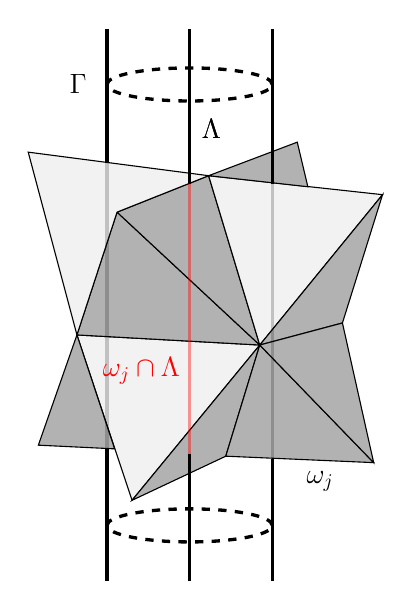
\begin{tikzpicture}[scale=0.7, every node/.style={scale=0.7}]
\pgfmathsetmacro{\factor}{1/sqrt(2)};
\coordinate  (A) at (2,0,-1*\factor);
\coordinate  (B) at (2.2,-1.2,2*\factor);
\coordinate  (C) at (-0.5,1,2*\factor);
\coordinate  (D) at (0.5,-2,2*\factor);
\coordinate  (E) at (0.5,3.5,3*\factor);
\coordinate  (F) at (0.8,2.8,-2*\factor);
\coordinate  (G) at (-1.2,-1,2*\factor);
\coordinate  (H) at (5.7,-0.5,5*\factor);
\coordinate  (I) at (1,-0.25,5*\factor);
\coordinate  (L) at (-2.5,3.2,-2.1*\factor);
\coordinate  (M) at (4.5,3,0*\factor);
\coordinate  (N) at (3.5,0.4,-1*\factor);
\coordinate  (O) at (2,3,-3.5*\factor);
\coordinate  (P) at (2.6,2.6,-2*\factor);
%\draw[->] (0,0) -- (3,0,0) node[right] {$x$};
%\draw[->] (0,0) -- (0,3,0) node[above] {$y$};
%\draw[->] (0,0) -- (0,0,3) node[below left] {$z$};
%\foreach \i in {A,B,C,D}
%\draw[dashed] (0,0)--(\i);
\draw[black, fill=white!90!gray] (A)--(D)--(C)--cycle;
\draw[black,  fill=gray!60!] (A) --(B)--(D)--cycle;
\draw[black, fill=gray!60!] (E) --(C)--(A)--cycle;
\draw[black,   fill=gray!60!] (E) --(F)--(A)--cycle;
\draw[black,    fill=gray!60!] (B) --(A)--(H)--cycle;
\draw[black,    fill=gray!60!] (C) --(G)--(I)--cycle;
\draw[black, fill=white!90!gray] (C) -- (E) -- (F)--(L)--cycle;
\draw[black,  fill=white!90!gray] (A) --(F)--(M)--cycle;
\draw[black,   fill=gray!60!] (A) --(N)--(M)--cycle;
\draw[black,    fill=gray!60!] (A) --(N)--(H)--cycle;
\draw[black,    fill=gray!60!] (F) --(O)--(P)--cycle;
%\draw[-, fill=gray!30!blue, opacity=.2] (E) --(G)--(H)--cycle;
\node [font=\Large, right] at (3, -2.2) {$\omega_j$};


%cylinder Gamma
\draw[dashed, very thick] (1, 5) ellipse (1.5 and 0.3);
\draw[dashed, very thick] (1, -3) ellipse (1.5 and 0.3);
\draw[black, very  thick] (-0.5, 3.6) -- (-0.5, 6);
\draw[black, very thick, opacity=.2] (-0.5, 3.6) -- (-0.5, -1.6);
\draw[black, very  thick] (-0.5, -1.6) -- (-0.5, -4); 
\draw[ very thick] (2.5, 6) -- (2.5, 3.2);
\draw[ very thick, opacity =0.2] (2.5, 3.2) -- (2.5, -1.8);
\draw[very thick] (2.5, -1.8) -- (2.5, -4);
\node [font=\Large, right] at (-1.3, 5) {$\Gamma$};

%centerline \Lambda
\draw[very thick] (1, 6) -- (1, 3.2);
\draw[red, very thick, opacity=.4] (1, 3.2) -- (1, -1.8);
\draw[very thick, ]  (1, -1.7) -- (1, -4);
\node [font=\Large, right] at (1.1, 4.2) {$\Lambda$};
\node [font=\Large, right] at (1.1, 4.2) {$\Lambda$};
\node [font=\Large, right, red] at (-0.7, -0.2) {$\omega _j \cap \Lambda$};
\end{tikzpicture}



%\end{document}
\caption{Extended patches $\omega_j$.}
\end{figure}

Moreover, we associate to each patch $\patch$ a shape-regular extended patch, still denoted by $\omega_j$ for notational simplicity, which is built adding to $\patch$ a sufficient number of elements of $\mathcal{T}_h^{\Omega}$ and we assume that the interiors of the new extended patches $\omega _j$ are still disjoint (see Figure \ref{fig:patch}). Here we are using the classical definition of shape-regularity, see for example \cite{MR2050138}, namely there exist a constant $C>0$ such that for any $\omega_j$, $\frac{\tilde{\rho}_j}{\bar{\rho}_j}\leq C$, being $\tilde{\rho}_j$ the diameter of $\omega_j$ and $\bar{\rho}_j$ the diameter of the largest ball that can be inscribed in $\omega_j$. The extended patches $\omega _j$ are built such that they fulfill the conditions meas$(\patch)=\mathcal{O}(H^3)$ and {\color{red}diam$(\Gamma_{\patch\cap \Lambda}\cap \omega_j)=O(H)$}, where $\Gamma_{\patch\cap \Lambda}$ is the portion of $\Gamma$ with centerline $\patch\cap \Lambda$. See Figure \ref{fig:gamma_generated} for a representation in the simple case in which $\omega _j$ is composed just by one tetrahedron. The latter assumption is required to ensure that the intersection of $\Gamma_{\patch\cap \Lambda}$ and $\omega_j$ is not too small and it will be needed later on to prove the inf-sup stability of the space $L_h$ in Lemma \ref{lemma:Lh_infsup}. We equipe the space $L_h$ with the discrete norm 
\begin{equation*}
\|\lld \|_{L_h} = \|\lld \|_{-\frac 12, h, \Lambda} = \|h^{\frac 12} \  \lld \|_{L^2(\Lambda)}.
\end{equation*}
As shown in \cite[Section III]{burman2014}, we can always choose $\pi_L$ as the $L_2$ orthogonal projection operator from $\Lambda_h$ to $L_h$ in order to satisfy \eqref{condition_pi_L} and then in practice replace it with any interpolation $\tilde{\pi}_L$ of $\Lambda_h$ in $L_h$. In particular, we define $\forall \lambda_h \in \Lambda_h$,
\begin{equation*}
\tilde{\pi}_L {\ld}_{ _{|\patch}} = N_j^{-1} \sum_{\substack{i: \ K_i \in \mathcal{G}_h, \  K_i \cap \omega_j \neq \emptyset}} {\ld}_{|K_i} \qquad \text{for all $\omega_j$,} 
\end{equation*}
being $N_j$ the cardinality of the set $\{i: \ K_i \in \mathcal{G}_h, \  K_i \cap \omega_j \neq \emptyset\}$. These choice leads to the following stabilization 
\begin{equation*}
s({\ld}_h, {\md}_h)= \sum _{K\in \mathcal{G}_{h}} \int_{\partial K\setminus \partial \mathcal{G}_{h}} h \llbracket {\ld}_h \rrbracket \llbracket {\md}_h \rrbracket,
\end{equation*}
being $\llbracket {\ld}_h \rrbracket$ the jump of ${\ld}_h$ across the internal faces of $\mathcal{G}_h$.

\begin{figure}\label{fig:gamma_generated}
\centering
\subfigure[$\Gamma_{\omega_j \cap \Lambda}$]
{
%\documentclass[tikz,border=3mm]{standalone}
%\usetikzlibrary{calc}
%\usetikzlibrary{shapes, snakes, patterns, arrows}
%\begin{document}

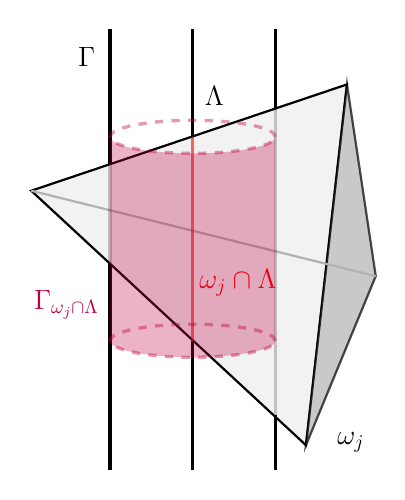
\begin{tikzpicture}[scale=0.7, every node/.style={scale=0.7}]
\pgfmathsetmacro{\factor}{1/sqrt(2)};


\coordinate  (A) at (-2.5,1.5,-2.1*\factor);
\coordinate  (B) at (3.8,4,0*\factor);
\coordinate  (C) at (3.6,-2,2*\factor);
\coordinate  (D) at (6.5,2.7,8*\factor);
\draw[thick, black,    fill=white!90!gray, opacity=1] (A) --(B)--(C)--cycle;
\draw[ thick,black,  fill=gray!60!, opacity=0.7] (D) --(B)--(C)--cycle;
\draw[thick,gray!60!] (D) --(A);
\node [font=\Large, right] at (3.5, -2.5) {$\omega_j $};


%cylinder Gamma
%\draw[dashed, very thick] (1, 5) ellipse (1.5 and 0.3);
%\draw[dashed, very thick] (1, -3) ellipse (1.5 and 0.3);
\draw[black, very  thick] (-0.5, 2.55) -- (-0.5, 5);
\draw[black, very thick, opacity=.2] (-0.5, 2.55) -- (-0.5, 0.75);
\draw[black, very  thick] (-0.5, 0.75) -- (-0.5, -3); 
\draw[ very thick] (2.5, 5) -- (2.5, 3.55);
\draw[ very thick, opacity =0.2] (2.5, 3.55) -- (2.5, -2);
\draw[very thick] (2.5, -2) -- (2.5, -3);
\node [font=\Large, right] at (-1.2, 4.5) {$\Gamma$};


%centerline \Lambda
\draw[very thick] (1, 5) -- (1, 3.05);
\draw[red, very thick, opacity=.6] (1, 3.05) -- (1, -0.65);
\draw[very thick, ]  (1, -0.65) -- (1, -3);
\node [font=\Large, right] at (1.1, 3.8) {$\Lambda$};
\node [font=\Large, right, red] at (1, 0.4) {$\omega _j \cap \Lambda$};

\draw[dashed, very thick, purple, opacity=.4] (1, 3.05) ellipse (1.5 and 0.3);
\draw[dashed, very thick, purple, opacity=.4] (1, -0.65) ellipse (1.5 and 0.3);

\fill [purple, opacity=0.3]  (-0.5, -0.65) arc (180:360:1.5 and 0.3) -- (2.5, 3.05) arc (0:180:1.5 and -0.3);
\node [font=\Large, right, purple] at (-2, 0) {$\Gamma_{\omega_j \cap \Lambda}$};

\end{tikzpicture}

%\end{document}
}
\qquad \qquad
\subfigure[ $\Gamma_{\omega_j \cap \Lambda} \cap \omega_j$]{
%\documentclass[tikz,border=3mm]{standalone}
%\usetikzlibrary{calc}
%\usetikzlibrary{shapes, snakes, patterns, arrows}
%\begin{document}
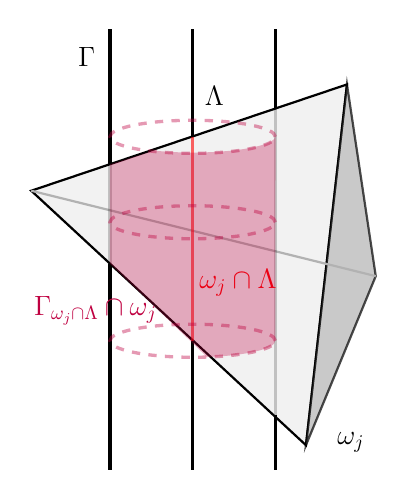
\begin{tikzpicture}[scale=0.7, every node/.style={scale=0.7}]

\pgfmathsetmacro{\factor}{1/sqrt(2)};

%tetrahedron
\coordinate  (A) at (-2.5,1.5,-2.1*\factor);
\coordinate  (B) at (3.8,4,0*\factor);
\coordinate  (C) at (3.6,-2,2*\factor);
\coordinate  (D) at (6.5,2.7,8*\factor);
\draw[thick, black,    fill=white!90!gray, opacity=1] (A) --(B)--(C)--cycle;
\draw[ thick,black,  fill=gray!60!, opacity=0.7] (D) --(B)--(C)--cycle;
\draw[thick,gray!60!] (D) --(A);
\node [font=\Large, right] at (3.5, -2.5) {$\omega_j $};


%cylinder Gamma
%\draw[dashed, very thick] (1, 5) ellipse (1.5 and 0.3);
%\draw[dashed, very thick] (1, -3) ellipse (1.5 and 0.3);
\draw[black, very  thick] (-0.5, 2.55) -- (-0.5, 5);
\draw[black, very thick, opacity=.2] (-0.5, 2.55) -- (-0.5, 0.75);
\draw[black, very  thick] (-0.5, 0.75) -- (-0.5, -3); 
\draw[ very thick] (2.5, 5) -- (2.5, 3.55);
\draw[ very thick, opacity =0.2] (2.5, 3.55) -- (2.5, -2);
\draw[very thick] (2.5, -2) -- (2.5, -3);
\node [font=\Large, right] at (-1.2, 4.5) {$\Gamma$};

%centerline \Lambda
\draw[very thick] (1, 5) -- (1, 3.05);
\draw[red, very thick, opacity=.6] (1, 3.05) -- (1, -0.65);
\draw[very thick, ]  (1, -0.65) -- (1, -3);
\node [font=\Large, right] at (1.1, 3.8) {$\Lambda$};
\node [font=\Large, right, red] at (1, 0.4) {$\omega _j \cap \Lambda$};

%intersection
\draw[dashed, very thick, purple, opacity=.4] (1, 3.05) ellipse (1.5 and 0.3);
\draw[dashed, very thick, purple, opacity=.4] (1, -0.65) ellipse (1.5 and 0.3);
\draw[dashed, very thick, purple, opacity=.4] (1, 1.5) ellipse (1.5 and 0.3);
\fill [purple, opacity=0.3]  (2.5, -0.65) arc (360:280:1.5 and 0.3) -- (-0.5, 0.75) -- (-0.5, 2.55) -- (0.3, 2.8) arc (118:0:1.5 and -0.3);
\node [font=\Large, right, purple] at (-2, -0.1) {$\Gamma_{\omega_j \cap \Lambda} \cap \omega_j$};

\end{tikzpicture}

%\end{document}
}
\caption{$\Gamma_{\omega_j \cap \Lambda}$, the portion of $\Gamma$ generated by $\omega_j \cap \Lambda$ in (a) and the intersection between $\Gamma_{\omega_j \cap \Lambda}$ and $\omega_j$ in (b). Here for simplicity $\omega_j$ is represented as a single tetrahedron but actually it is a collection of tetrahedra as shown in Figure \ref{fig:patch}.}
\end{figure}
Thanks to the shape regularity of these extended patches, we have that the following discrete trace and Poincarè-type inequalites hold. More precisely, for any function $v\in H^1(\omega_j)$, 
\begin{equation}\label{discr_trace_ineq}
\|\trace v\|_{L^2(\Gamma\cap \omega_j)} \lesssim H^{-\frac 12} \|v\|_{L^2(\omega_j)}
\end{equation}
\begin{equation}\label{disc_poincare_ineq}
\|v- \mathcal{E}_{\patch} \pi_L\mtrace v\|_{L^2(\omega_j)} \leq c_P H \|\nabla v\|_{L^2(\omega_j)},
\end{equation}
%where $\pi_L$ is a projection operator onto piecewise constant functions on $\patch\cap \Lambda$. In particular, for any $w \in L^2(\Lambda)$, we define
where for any $w \in L^1(\Lambda)$, $ \mathcal{E}_{\patch}\pi_Lw \in L_h$ and with a little abuse of notation we denote as $\pi_L$ the operator
\begin{equation*}
\pi_Lw_{|\patch \cap \Lambda} =\frac{1}{|\Gamma_{\patch\cap \Lambda}|}\int_{\patch\cap \Lambda}|\DD| w\quad \forall j,
\end{equation*}   
whereas the operator $\mathcal{E}_{\patch}$ simply extends the constant $\pi_L\mtrace v_{|\patch \cap \Lambda}$ to $\omega _j$.
Moreover $\forall u_h \in X^1_{h,0}(\Omega)$ we have the following average inequality 
\begin{equation*}
\sum _j \|\mtrace u_h\|^2_{L^2(\patch \cap \Lambda),|\DD| } \leq \sum _j \|\trace  u_h\|^2_{L^2(\omega_j\cap \Gamma)}.
\end{equation*}
Indeed, by the definition of $\mtrace$ and Jensen inequality, we have
\begin{multline*}
\sum _j \|\mtrace u_h\|^2_{L^2(\patch \cap \Lambda),|\DD| }
= \sum _j\int_{\patch \cap \Lambda} |\DD| \mtrace u_h^2 
\\
= \int_{\Lambda} |\DD| \left( \frac{1}{|\DD|} \int_{\DD} \trace u_h \right)^2
\\
(\text{Jensen})\leq \int_{\Lambda} \int_{\DD} (\trace u_h)^2
= \int_{\Gamma} (\trace u_h)^2
\\
(\patch \cap \Gamma \text{ partition of } \Gamma)= \sum _j \int_{\patch \cap \Gamma} (\trace u_h)^2
= \sum _j \|\trace u_h\|^2_{L^2(\patch \cap \Gamma)}.
\end{multline*}

\begin{lemma}\label{lemma:Lh_infsup}
The space $L_h$ is inf-sup stable, namely $\forall {\lld}_h \in L_h$, $\exists \beta >0$ s.t.
\begin{equation*}
\sup_{\substack{v_h \in X_{h,0}^1(\Omega),\\ {\vd}_h \in X_{h',0}^1(\Lambda)}} \frac{\left(\mtrace v_h - {\vd}_h, {\lld} _h\right)_{\Lambda, |\DD|}}{\vertiii{[v_h, {\vd}_h]}} \geq \beta \|{\lld}_h\|_{H^{-\frac 12}(\Lambda)}.
\end{equation*} 
and the constant is independent of the cuts. 
\end{lemma}
\begin{proof}
% We have to prove that $\exists \beta >0$ such that $\forall l_h \in L_h$,
%\begin{equation*}
%\sup_{\substack{v_h \in X_{h,0}^1(\Omega),\\ {\vd}_h \in X_{h',1}^0(\Lambda)}} \frac{\left(\avrc{T v_h} - {\vd}_h, l _h\right)_{\Lambda, |\DD|}}{\vertiii{[v_h, {\vd}_h]}} \geq \beta \|l_h\|_{H^{-\frac 12}(\Lambda)}.
%\end{equation*}
As in the continuous case, we can choose ${\vd}_h=0$ and we prove that
\begin{equation*} 
\sup_{v_h \in X_{h,0}^1(\Omega)} \frac{\left(\mtrace v_h ,{\lld}_h\right)_{\Lambda, |\DD|}}{\|v_h\|_{H^1(\Omega)}} \geq \beta \|{\lld}_h\|_{H^{-\frac 12}(\Lambda)}.
\end{equation*} 
Proving the last inequality it is equivalent to find the Fortin operator $\pi_F: H^1_0(\Omega) \rightarrow X_{h,0}^1(\Omega)$, such that 
\begin{equation*}
\left(\mtrace v - \mtrace \pi _F v  , {\lld}_h\right)_{\Lambda, |\DD|}=0, \quad \forall v\in H^1_0(\Omega), \, {\lld}_h \in L_h
\end{equation*} 
and
\begin{equation*}
\|\pi_F v\|_{H^1(\Omega)}\lesssim \|v\|_{H^1(\Omega)}.
\end{equation*} 

We define
\begin{equation*}
\pi_F v = I_h v + \sum _j \alpha _j \varphi _j \qquad \text{with }\alpha_j =\frac{\int_{\patch \cap \Lambda}|\DD| (\mtrace v-\mtrace I_h v)}{\int_{\patch \cap \Lambda}|\DD|\mtrace \varphi _j}
\end{equation*}
where $I_h: H^1(\Omega) \rightarrow X_{h,0}^1$ denotes an $H^1(\Omega)$-stable interpolant
and $\varphi_j \in X_{h,0}^1(\Omega)$ is such that supp$(\varphi_j)\subset \omega_j$, supp$(\trace \varphi _j) \subset \Gamma_{\patch\cap \Lambda}\cap \omega_j$, $\varphi_j =0$ on $\partial \omega _j$ and 
\begin{equation}\label{phi_properties}
 {\color{red}\int_{\patch\cap \Lambda}|\DD|\mtrace \varphi_j=O(H)} \text{ and } \|\nabla \varphi _j\|_{L^2(\omega _j)}=O(1). 
\end{equation}
We notice that supp$(\trace \varphi_j) \subset \Gamma_{\patch\cap \Lambda}\cap \omega_j$ ensures that $\mtrace \varphi_j \subset \omega_j\cap \Lambda$. Therefore, since for construction the interiors of $\omega_j\cap \Lambda$  are disjoint and $\varphi _j = 0 $ on $\partial \omega_j$,  the functions $\mtrace \varphi_j\, \forall j$ have all disjoint supports. This construction is always possible since meas$(\patch) = \mathcal{O}(H^3)$ and diam$(\Gamma_{\patch\cap \Lambda} \cap \omega_j)=\mathcal{O}(H)$, provided $H$ is sufficiently larger that $h$. Indeed, this guarantees that the functions $\varphi _j$ and their traces $\trace \varphi _j$ have a sufficiently large support so that they can be built in order to satisfy \eqref{phi_properties}.
Then we have
\begin{multline*}
\left(\mtrace v - \mtrace \pi _F v  , {\lld}_h\right)_{\Lambda, |\DD|} = \sum _j \int_{\patch\cap \Lambda} |\DD |\left[ \mtrace v-\mtrace I_h v-\sum _i \alpha_i \mtrace \varphi _i \right]{\lld}_h \\
(\text{supp} (\mtrace \varphi _i )\subset \omega _i\cap \Lambda \, \forall i)  =\sum _j \int_{\patch\cap \Lambda}|\DD| \left[ \mtrace v-\mtrace I_h v-\alpha_j \mtrace \varphi _j \right]{\lld}_h\\
=\sum _j \int_{\patch\cap \Lambda} |\DD| (\mtrace v-\mtrace  I_h v) {\lld}_h - \frac{\int_{\patch\cap \Lambda} |\DD| (\mtrace v-\mtrace I_h v)}{\int_{\patch\cap \Lambda}|\DD|\mtrace \varphi _j} \int_{\patch\cap \Lambda} |\DD|\mtrace \varphi _j{\lld}_h\\ 
(\text{using $l_h$ constant on $\patch\cap \Lambda$})=0.
\end{multline*}
Concerning the continuity of $\pi_F$, we exploit the assumptions that the interiors of $\patch$ are disjoint and supp$(\varphi _j) \subset \patch$ and we have
\begin{multline*}
\|\nabla \pi_F v \|_{L^2(\Omega)} \leq \|\nabla I_h v\|_{L^2(\Omega)} + \left(\sum_j\alpha_j^2\|\nabla \varphi _j\|^2_{L^2(\omega_j)}\right)^{\frac 12}\\
(\text{stability of }I_h)\lesssim   \|\nabla  v\|_{L^2(\Omega)} + \left(\sum_j\alpha_j^2\|\nabla \varphi _j\|^2_{L^2(\omega_j)}\right)^{\frac 12}
\end{multline*}
and for the second term 
\begin{multline*}
\sum_j \alpha_j ^2\|\nabla \varphi _j\|^2_{L^2(\omega_j)}\leq
\\
\left(\text{using }\|\nabla \varphi _j\|_{{L^2(\omega_j)}}=O(1)\right) \lesssim  \sum_j \frac{\left(\int_{\patch\cap \Lambda} |\DD| (\mtrace v-\mtrace I_h v)\right)^2}{\left(\int_{\patch\cap \Lambda}|\DD|\mtrace \varphi_j \right)^2}
\\
\left(\text{since }\int_{\patch\cap \Lambda}|\DD|\mtrace \varphi_j=O(H)\right) \lesssim \frac {1}{H^2} \sum_j \left(\int_{\patch\cap \Lambda} |\DD| (\mtrace v-\mtrace I_hv)\right)^2
\\
(\text{Jensen}) \lesssim  \frac {1}{H^2} \sum_j |\patch\cap \Lambda| \int_{\patch\cap \Lambda} |\DD|^2(\mtrace v-\mtrace I_h v)^2
\\
(\text{being }|\patch\cap \Lambda| \leq cH)\lesssim  \frac {1}{H} \sum_j \| \mtrace (v-I_h v)\|^2_{L^2(\patch\cap \Lambda), |\DD|}
\\
(\text{average inequality}) \lesssim  \frac {1}{H} \sum_j \| \trace(v-I_h v)\|^2_{L^2(\omega _j\cap \Gamma)}  
\\
\left(\text{trace inequality} \right)\lesssim  \frac {1}{H^2} \sum_j  \| v-I_h v\|^2_{L^2(\omega_j)} \lesssim  \frac {1}{H^2}  \| v-I_h v\|^2_{L^2(\Omega)} 
\\
(\text{approximation properties of }I_h)\lesssim \|\nabla  v\|^2_{L^2(\Omega)}
\end{multline*}
and the continuity of $\pi_F$ follows.
\end{proof}

%\subparagraph{Satisfaction of the assumptions of the 
%abstract analysis}
We choose the following discrete norm
\begin{equation*}
\vertiii{[u_h, {\ud}_h]}^2_{X_h(\Omega)\times X_{h'}(\Lambda) }
= \|u_h\|^2_{H^1(\Omega)}+\|{\ud}_h\|^2_{H^1(\Lambda),|\D|} + \|\mtrace u_h - {\ud}_h\|^2_{\frac 12, h, \Lambda, |\DD|},
\end{equation*}
where $\|\mtrace u_h - {\ud}_h\|^2_{\frac 12, h, \Lambda, |\DD|} = \|h^{-\frac 12} (\mtrace u_h - {\ud}_h)\|^2_{L^2(\Lambda), |\DD|} $. Then, we have the following lemma. 
\begin{lemma}
The inequalities \eqref{stab_coercivity} and \eqref{stab_stability} hold.
\end{lemma}
\begin{proof} 
Concerning the coercivity property \eqref{stab_coercivity}, we have to show that $\forall [u_h, {\ud}_h]$, there esists $\xi_h \in Q_h$ s.t.
\begin{multline*}
(u_h,u_h)_{H^1(\Omega)}+ ({\ud}_h, {\ud}_h)_{H^1(\Lambda), |\D|} +   (\mtrace u_h - {\ud}_h, \xi_h)_{\Lambda,|\DD|} \\
\geq \alpha_{\xi}(\|u_h\|^2_{H^1(\Omega)}+\|{\ud}_h\|^2_{H^1(\Lambda),|\D|}+ \|\mtrace u_h - {\ud}_h\|^2_{\frac 12, h, \Lambda, |\DD|}.
\end{multline*}
We choose 
\begin{equation*}
{\xi_h}_{|\patch\cap \Lambda}=\delta \frac 1H \pi_L(\mtrace u_h-{\ud}_h)_{|\patch \cap \Lambda}
\end{equation*}
and we recall that 
\begin{equation*}
\pi_L(\mtrace u_h-{\ud}_h)_{|\patch \cap \Lambda}=\frac{1}{|\Gamma_{\patch\cap \Lambda}|}\int_{\patch\cap \Lambda}|\DD| (\mtrace u_h- {\ud}_h).
\end{equation*} 
Actually, $\mathcal{E}_{\patch}\xi_h\in L_h \subset Q_h$. Then,
\begin{multline*}
\left( \mtrace u_h - {\ud}_h, \xi _h \right)_{\Lambda,|\DD|} 
= \sum_j \int_{\patch\cap \Lambda} |\DD|(\mtrace u_h - {\ud}_h)\xi_h
\\
(\text{definition of $\xi_h$})= \delta \frac{1}{H}\sum_j \pi_L( \mtrace u_h - {\ud}_h)\int_{\patch\cap \Lambda} |\DD|(\mtrace u_h - {\ud}_h)
\\
= \delta \frac{1}{H} \sum_j \int_{\patch\cap \Lambda}|\DD| (\pi_L( \mtrace u_h - {\ud}_h) )^2
\\
(\text{orthogonality of $\pi_L$}) = - \delta \frac{1}{H} \|(\pi_L-\mathcal{I})(\mtrace u_h - {\ud}_h)\|^2_{L^2(\patch\cap \Lambda),|\DD|} + \delta \frac{1}{H} \|\mtrace u_h - {\ud}_h\|^2_{L^2(\patch\cap \Lambda),|\DD|}
\\ 
\geq -2\delta \frac 1H \sum_j \|(\pi_L - \mathcal{I})\mtrace u_h\|^2_{L^2(\patch\cap \Lambda), |\DD|}
-2 \delta \frac 1H \sum_j \|(\pi_L - \mathcal{I}){\ud}_h\|^2_{L^2(\patch\cap \Lambda),|\DD|}
\\ 
+ \delta \frac 1H \sum_j \|\mtrace u_h-{\ud}_h\|^2_{L^2(\patch\cap \Lambda),|\DD|}. 
\end{multline*}
For the first term we have
\begin{multline*}
\sum _j  \|(\pi_L - \mathcal{I})\mtrace u_h\|^2_{L^2(\patch\cap \Lambda),|\DD|} =\sum _j \int _{\patch \cap \Lambda} |\DD| (\pi_L \mtrace u_h- \mtrace u_h)^2
\\
(\text{Average inequality)} \leq \sum _j  \int_{\omega _j \cap \Gamma} (\ext \pi_L \mtrace u_h -\trace u_h)^2 
\\
(\text{trace inequality}) \leq \sum _j  \frac 1H \int_{\omega_j}(\mathcal{E}_{\patch} \pi_L \mtrace u_h - u_h)^2 
\\ 
(\text{Poincare, see \cite[Corollary B.65]{MR2050138}})\leq \sum _j  H c_P ^2 \|\nabla u_h\|^2_{L^2(\omega _j)}.
\end{multline*}
For the second term we have
\begin{multline*}
\sum _j \|(\pi_L - \mathcal{I}){\ud}_h\|^2_{L^2(\patch\cap \Lambda),|\DD|} = \sum _j \int_{\patch\cap \Lambda} |\DD| (\pi_L {\ud}_h -{\ud}_h)^2
\\
(\text{Poincare, \cite[Corollary B.65]{MR2050138}})\lesssim \sum _j  H^2 c_P^2 \int_{\patch\cap \Lambda} |\DD|(\nabla {\ud}_h)^2
\\
(\text{since $H$ is fixed, we can find a constant s.t. } H|\DD| \lesssim |\D|) \lesssim \sum _j H c_P^2  \int_{\patch\cap \Lambda} |\D|(\nabla {\ud}_h)^2 
\\
\lesssim \sum _j H c_P^2  \|\nabla {\ud}_h\|^2_{L^2(\patch\cap \Lambda),|\D|}.
\end{multline*}
%{\color{red} N.B. we are using a kind of weigthed Poincare inequality, check... I think it should work because I can do something like this
%\begin{multline*}
%\int_{\patch \cap \Lambda} |\DD| u^2 \leq 
%max |\DD| \int_{\patch \cap \Lambda} u^2 \leq
%max |\DD| \int_{\patch \cap \Lambda} (\nabla u)^2 =
%\frac{max |\DD|}{min|\DD|} min|\DD| \int_{\patch \cap \Lambda} (\nabla u)^2 \leq\\
%\frac{max |\DD|}{min|\DD|}  \int_{\patch \cap \Lambda} |\DD| (\nabla u)^2 
%\end{multline*}
%}\\
Therefore, we obtain
\begin{multline*}
a([u_h, {\ud}_h],[u_h, {\ud}_h] ) + b([u_h, {\ud}_h], \xi_h([u_h, {\ud}_h]))
\geq \\
(1-2\delta c_P^2) \|\nabla u_h\|^2_{L^2(\Omega)} + (1- 2\delta c_P^2) \|\nabla {\ud}_h\|^2_{L^2(\Lambda), |\D|}
+\delta c_H  \|\mtrace u_h-{\ud}_h\|^2_{\frac 12,h,\Lambda, |\DD|}
\end{multline*}
and choosing $\delta=\frac{1}{4c_P^2}$ we obtain the coercivity inequality.\\
Concerning the stability inequality \eqref{stab_stability}, the proof is analogous to the one in \cite{burman2014}.
\end{proof}

\begin{remark}
We notice that if we choose $Q_h=X_{h',0}^1(\Lambda)$, the constant in the inf-sup inequality  \eqref{eq:infsup_discrete} depends on the mesh size $h'$. Indeed,
\begin{multline}
\sup_{\substack{v_h \in X_{h,0}^1(\Omega),\\ {\vd}_h \in X_{h',0}^1(\Lambda)}} \frac{\left(\mtrace v_h - {\vd}_h, {\lld} _h\right)_{\Lambda, |\DD|}}{\vertiii{[v_h, {\vd}_h]}}
\geq \sup_{\substack{{\vd}_h \in X_{h',0}^1(\Lambda)}} \frac{\left(- {\vd}_h, {\lld} _h\right)_{\Lambda, |\DD|}}{\|{\vd}_h\|_{H^1(\Lambda)}}
\geq \frac{{\|\lld} _h\|^2_{L^2(\Lambda)}}{\|{\vd}_h\|_{H^1(\Lambda)}} \\
( \text{inverse inequality} )\geq \frac{{h'}^2}{c_I} \|{\lld}_h\|_{L^2(\Lambda)}
\geq  \frac{{h'}^2}{c_I} \|{\lld}_h\|_{H^{-\frac 12},(\Lambda)}
\end{multline}
being $c_I$ the constant in the inverse inequality
\begin{equation*}
\|{\lld}_h\|_{H^1(\Lambda)} \leq \frac{c_I} {{h'}^2} \|{\lld}_h\|_{L^2(\Lambda)}. 
\end{equation*}
\end{remark}


%>>>>>>>>>>>>>>>>>>>>>>>>>>>>>>>>>>>>>>>>>>>>>>>>>>

\section{A benchmark problem with analytical solution}

We consider the following 3D-1D coupled problem,
\begin{subequations}\label{benchmark}
\begin{align}
\label{benchm_3d}
-\Delta u=f \quad &\text{in $\Omega$}\\
\label{benchm_1d}
-d_{zz}^2 \ud =g \quad &\text{on $\Lambda$}\\
u=0 \quad &\text{on $\partial \Omega$}\\
\label{benchm_coupl}
\ud -\avrc{u}=q \quad &\text{on $\Lambda$}
\end{align}
\end{subequations}

where $\Omega=[0,1]\times [0,1]\times [0,H]$, $\Lambda=\{x=0.5\}\times \{y=0.5\} \times [0,H] $ and
\begin{eqnarray*}
f=8\pi ^2 \sin (2\pi x) \sin (2\pi y)\\
%g=-\exp(-z)\\
%q=1+\exp(-z).
g=\frac{\pi ^2}{H^2} \sin \left(\frac{\pi z}{H}\right)\\
q=\sin \left(\frac{\pi z}{H}\right).
\end{eqnarray*}
In this case the $z$ coordinate coincides with the axial coordinate along $\Lambda$. We define $\Sigma=[0.25,0.75]\times [0.25,0.75]\times [0,H]$. The average of the 3D solution $\avrc{u}$ in \eqref{benchm_coupl} is computed on the cross section $\DD$ of the virtual interface $\Gamma=\partial \Sigma$. The exact solution of \eqref{benchmark} is given by
\begin{eqnarray}
\label{benchm_sol3d}
u=\sin (2\pi x) \sin (2\pi y)\\
\label{benchm_sol1d}
%\ud=1+\exp(-z).
\ud=\sin \left(\frac{\pi z}{H}\right) 
\end{eqnarray}
Let us notice that $\ud$ satisfies homogeneous Dirichlet conditions at the boundary of $\Lambda$.
Moreover, the solution \eqref{benchm_sol3d}-\eqref{benchm_sol1d} satisfies on $\Gamma$ the relation
\begin{equation}\label{benchm_flux}
\lambda=\nabla u \cdot \textbf{n}_{\oplus}=d_z \ud n_{\oplus,z}=0,
\end{equation}
being $n_{\oplus,z}$ the $z-$component of the normal unit vector to $\Gamma$.

We prove that \eqref{benchm_sol3d}-\eqref{benchm_sol1d} is solution of \eqref{eq:problem1} and \eqref{eq:problem2} in the simplified case in which the starting 3D-3D problem is
\begin{subequations}\label{eq:dirneu_simple}
\begin{align}
- \Delta \up  &= f  && \text{ in } \Omega_{\oplus},\\
- \Delta \uf &= g  && \text{ in } \Sigma,\\
-\nabla \uf \cdot \nn_{\ominus} &= -\nabla \up \cdot \nn_{\ominus}  && \text{ on } \Gamma,\\
\uf - \up &= q  && \text{ on }  \Gamma,\\
\up &= 0 && \text{ on } \partial \Omega\,.
\end{align}
\end{subequations}
instead of \eqref{eq:dirneu}. Therefore the reduced problems in the two different formulations \eqref{eq:problem1} and \eqref{eq:problem2} become respectively
 
\begin{subequations}\label{eq:problem1_simple}
\begin{align}
\label{eq:problem1_simple_eq1}
&(\nabla u,\nabla v)_{L^2(\Omega)} + |{\cal D}|(d_s \ud,d_s \vd)_{L^2(\Lambda)} 
+ \langle \Pi_1 v  - \Pi_2 \vd, L \rangle_\Gamma
\\
\nonumber
&\qquad\qquad= (f,v)_{L^2(\Omega)} + |{\cal D}| (\avrd{g},\vd)_{L^2(\Lambda)}
\quad \forall v \in H^1_0(\Omega), \ \vd \in H^1(\Lambda)
\\
\label{eq:problem1_simple_eq2}
&   \langle \Pi_1 u - \Pi_2 \ud , M \rangle_\Gamma =  \langle q , M \rangle_\Gamma
\quad \forall M \in H^{-\frac12}(\Gamma)\,.
\end{align}
\end{subequations}

and

\begin{subequations}\label{eq:problem2_simple}
\begin{align}
&(\nabla u,\nabla v)_{L^2(\Omega)} + |{\cal D}|(d_s \ud,d_s \vd)_{L^2(\Lambda)} 
+ |\partial {\cal D}| \langle \Pi_1 v - \Pi_2 \vd, L \rangle_{H^{-\frac12}(\Lambda)} 
\\
\nonumber
&\qquad\qquad= (f,v)_{L^2(\Omega)} + |{\cal D}| (\avrd{g},V)_{L^2(\Lambda)}
\quad \forall v \in H^1_0(\Omega), \ \vd \in H^1_0(\Lambda)
\\
&  |\partial {\cal D}| \langle \Pi_1 u -  \Pi_2 \ud, M \rangle_{H^{-\frac12}(\Lambda)} =|\partial {\cal D}| \langle \avrc{q}, M \rangle_{H^{-\frac12}(\Lambda)}
\quad \forall M \in H^{-\frac12}(\Lambda)\,.
\end{align}
\end{subequations}

Let us prove that \eqref{benchm_sol3d}-\eqref{benchm_sol1d} is solution of \eqref{eq:problem1_simple}. Using the integration by part formula and homogeneous boundary conditions on $\Omega$ and $\Lambda$, from \eqref{eq:problem1_simple_eq1} we have
\begin{align*}
&-(\Delta u, v)_{L^2(\Omega)} - |{\cal D}|(d^2_{ss} \ud, \vd)_{L^2(\Lambda)} 
+ \langle \Pi_1 v  - \Pi_2 \vd, L \rangle_\Gamma
\\
\nonumber
&\qquad\qquad= (f,v)_{L^2(\Omega)} + |{\cal D}| (\avrd{g},\vd)_{L^2(\Lambda)}
\quad \forall v \in H^1_0(\Omega), \ \vd \in H^1(\Lambda).
\\
\end{align*}
Clearly, since \eqref{benchm_sol3d} satisfies \eqref{benchm_3d} and \eqref{benchm_sol1d} satisfies \eqref{benchm_1d}, we have that \begin{align*}
-(\Delta u, v)_{L^2(\Omega)} =  (f,v)_{L^2(\Omega)} \\
-|{\cal D}|(d^2_{ss} \ud, \vd)_{L^2(\Lambda)}  = |{\cal D}| (\avrd{g},\vd)_{L^2(\Lambda)}
\end{align*}
and being $L=\lambda=0$, we can conclude that \eqref{benchm_sol3d}-\eqref{benchm_sol1d} satisfy \eqref{eq:problem1_simple_eq1}. The fact that the solution satisfy \eqref{eq:problem1_simple_eq2} follows from \eqref{benchm_coupl}. We can prove in the same way that \eqref{benchm_sol3d}-\eqref{benchm_sol1d} is solution of \eqref{eq:problem2_simple}, exploiting the fact that in this case $L=\avrc{\lambda}=0$. 

\begin{remark}
Let us notice that the 3D solution \eqref{benchm_sol3d} is such that $\avrc{u}=0$. Therefore in \eqref{benchmark} it is like we are solving two separated problems, one in $\Omega$ and the other on $\Lambda$.
\end{remark}
\begin{remark}
It would be interesting to make a comparison between the solution of the fully coupled 3D-3D problem \eqref{eq:dirneu} (also in the simplified case of type \eqref{eq:dirneu_simple}) and the solution of the reduced problems \eqref{eq:problem1} and \eqref{eq:problem2}. 
Therefore, we could set the values of the data of the problem such that the reduced formulation becomes non-trivial and fully coupled.
Then, we will solve both the original and reduced problem to observe the differences in the solutions and the values of the Lagrange multiplier.
\end{remark}

%-----------------
\bibliographystyle{siamplain}
\bibliography{3d1d_coupled}

\appendix
\section{System sizes in benchmark formulations}\label{sec:appendix}
Below we list dimensions of the finite element spaces used to discretize
formualations \eqref{eq:problem1}, \eqref{eq:problem2} and stabilized
\eqref{eq:problem2} on different levels of refinement.

\begin{center}
  \scriptsize{
    \begin{tabular}{l|lll|lll|lll}
      \toprule
      \multirow{2}{*}{$l$} & \multicolumn{3}{c|}{\eqref{eq:problem1}} & \multicolumn{3}{c|}{\eqref{eq:problem2}} & \multicolumn{3}{c}{ Stabilized \eqref{eq:problem2}}\\
      \cline{2-10}
      & $\lvert X^1_{h, 0}(\Omega) \rvert$ & $\lvert X^1_{h, 0}(\Lambda) \rvert$ & $\lvert Q_h(\Gamma) \rvert$ &
      $\lvert X^1_{h, 0}(\Omega) \rvert$ & $\lvert X^1_{h, 0}(\Lambda) \rvert$ & $\lvert Q_h(\Lambda) \rvert$ &
      $\lvert X^1_{h, 0}(\Omega) \rvert$ & $\lvert X^1_{h^{\prime}, 0}(\Lambda) \rvert$ & $\lvert Q_h(\mathcal{G}_h) \rvert$\\
      \hline
     1& 125    & 5  & 40   & 125     & 5   & 5   & 180     & 13  & 24  \\
     2& 729    & 9  & 144  & 729     & 9   & 9   & 900     & 25  & 48  \\
     3& 4913   & 17 & 544  & 4913    & 17  & 17  & 5508    & 49  & 96  \\
     4& 35937  & 33 & 2112 & 35937   & 33  & 33  & 38148   & 97  & 192 \\
     5& 274625 & 65 & 8320 & 274625  & 65  & 65  & 283140  & 193 & 384 \\
     6& --     & -- & -    & 2146689 & 129 & 129 & 2180100 & 385 & 768 \\
      \bottomrule
    \end{tabular}
    }
    \end{center}


\end{document}
